\documentclass[11pt]{article}

\usepackage[T1]{fontenc}
\usepackage[utf8]{inputenc}
\usepackage{lmodern}
\usepackage[margin=1in]{geometry}
\usepackage{amsmath,amssymb}
\usepackage{booktabs}
\usepackage{tabularx}
\usepackage{graphicx}
\usepackage[numbers,sort&compress]{natbib}
\usepackage{xcolor}
\usepackage[hidelinks]{hyperref}
\usepackage{url}

% Benchmark and field names, set in monospace with line breaks at slashes.
\newcommand{\bench}[1]{\nolinkurl{#1}}
\newcommand{\field}[1]{\texttt{#1}}
\newcommand{\file}[1]{\nolinkurl{#1}}

% Results numbers. Until the M4 run this file holds \textbf{??} placeholders with
% the macro names analysis/numbers.py emits. At M4, replace this line with
% % Generated by analysis.numbers from results/*.json. Do not edit.
\newcommand{\BenchAAnalysisRows}{2813}
\newcommand{\BenchAFirthMethod}{firth}
\newcommand{\BenchAFitRows}{2423}
\newcommand{\BenchALogOR}{0.157}
\newcommand{\BenchAName}{davidtai/mlxfast-gemma4-26b-a4b}
\newcommand{\BenchAOR}{1.170}
\newcommand{\BenchAORHigh}{1.737}
\newcommand{\BenchAORLow}{0.788}
\newcommand{\BenchAStrataDropped}{46}
\newcommand{\BenchAStrataKept}{40}
\newcommand{\BenchAStrataNoTreatmentVariation}{4}
\newcommand{\BenchBAnalysisRows}{5409}
\newcommand{\BenchBFirthMethod}{firth}
\newcommand{\BenchBFitRows}{4564}
\newcommand{\BenchBLogOR}{0.224}
\newcommand{\BenchBName}{davidtai/qwen38-125b-a6b-cuda-v1}
\newcommand{\BenchBOR}{1.251}
\newcommand{\BenchBORHigh}{2.141}
\newcommand{\BenchBORLow}{0.731}
\newcommand{\BenchBStrataDropped}{17}
\newcommand{\BenchBStrataKept}{21}
\newcommand{\BenchBStrataNoTreatmentVariation}{2}
\newcommand{\BenchCAnalysisRows}{1332}
\newcommand{\BenchCFirthMethod}{firth}
\newcommand{\BenchCFitRows}{894}
\newcommand{\BenchCLogOR}{0.502}
\newcommand{\BenchCName}{eigenlabs/eip8200-challenges/modexp}
\newcommand{\BenchCOR}{1.651}
\newcommand{\BenchCORHigh}{2.687}
\newcommand{\BenchCORLow}{1.015}
\newcommand{\BenchCStrataDropped}{16}
\newcommand{\BenchCStrataKept}{20}
\newcommand{\BenchCStrataNoTreatmentVariation}{2}
\newcommand{\BenchDAnalysisRows}{1073}
\newcommand{\BenchDFirthMethod}{firth}
\newcommand{\BenchDFitRows}{579}
\newcommand{\BenchDLogOR}{-0.122}
\newcommand{\BenchDName}{eigenlabs/eip8200-challenges/ripemd160}
\newcommand{\BenchDOR}{0.885}
\newcommand{\BenchDORHigh}{1.448}
\newcommand{\BenchDORLow}{0.541}
\newcommand{\BenchDStrataDropped}{11}
\newcommand{\BenchDStrataKept}{19}
\newcommand{\BenchDStrataNoTreatmentVariation}{0}
\newcommand{\BenchEAnalysisRows}{4605}
\newcommand{\BenchEFirthMethod}{firth}
\newcommand{\BenchEFitRows}{1785}
\newcommand{\BenchELogOR}{-0.291}
\newcommand{\BenchEName}{eigenlabs/flock-challenge}
\newcommand{\BenchEOR}{0.747}
\newcommand{\BenchEORHigh}{1.111}
\newcommand{\BenchEORLow}{0.503}
\newcommand{\BenchEStrataDropped}{20}
\newcommand{\BenchEStrataKept}{36}
\newcommand{\BenchEStrataNoTreatmentVariation}{9}
\newcommand{\BenchFAnalysisRows}{3240}
\newcommand{\BenchFFirthMethod}{firth}
\newcommand{\BenchFFitRows}{2360}
\newcommand{\BenchFLogOR}{-0.290}
\newcommand{\BenchFName}{eigenlabs/flock-challenge-multi/x86}
\newcommand{\BenchFOR}{0.748}
\newcommand{\BenchFORHigh}{1.468}
\newcommand{\BenchFORLow}{0.381}
\newcommand{\BenchFStrataDropped}{29}
\newcommand{\BenchFStrataKept}{19}
\newcommand{\BenchFStrataNoTreatmentVariation}{6}
\newcommand{\BenchGAnalysisRows}{8208}
\newcommand{\BenchGFirthMethod}{firth}
\newcommand{\BenchGFitRows}{6868}
\newcommand{\BenchGLogOR}{0.235}
\newcommand{\BenchGName}{eigenlabs/lighter-prover-challenge}
\newcommand{\BenchGOR}{1.265}
\newcommand{\BenchGORHigh}{1.913}
\newcommand{\BenchGORLow}{0.837}
\newcommand{\BenchGStrataDropped}{61}
\newcommand{\BenchGStrataKept}{46}
\newcommand{\BenchGStrataNoTreatmentVariation}{4}
\newcommand{\BenchHAnalysisRows}{1883}
\newcommand{\BenchHFirthMethod}{firth}
\newcommand{\BenchHFitRows}{1260}
\newcommand{\BenchHLogOR}{-0.443}
\newcommand{\BenchHName}{eigenlabs/mlxfast-challenge}
\newcommand{\BenchHOR}{0.642}
\newcommand{\BenchHORHigh}{1.088}
\newcommand{\BenchHORLow}{0.379}
\newcommand{\BenchHStrataDropped}{51}
\newcommand{\BenchHStrataKept}{32}
\newcommand{\BenchHStrataNoTreatmentVariation}{8}
\newcommand{\BenchIAnalysisRows}{685}
\newcommand{\BenchIFirthMethod}{firth}
\newcommand{\BenchIFitRows}{487}
\newcommand{\BenchILogOR}{0.466}
\newcommand{\BenchIName}{eigenlabs/sig-golf/full}
\newcommand{\BenchIOR}{1.594}
\newcommand{\BenchIORHigh}{2.696}
\newcommand{\BenchIORLow}{0.942}
\newcommand{\BenchIStrataDropped}{18}
\newcommand{\BenchIStrataKept}{23}
\newcommand{\BenchIStrataNoTreatmentVariation}{2}
\newcommand{\BenchJAnalysisRows}{1439}
\newcommand{\BenchJFirthMethod}{firth}
\newcommand{\BenchJFitRows}{417}
\newcommand{\BenchJLogOR}{-0.897}
\newcommand{\BenchJName}{gpsanant/ecdsafail-challenge}
\newcommand{\BenchJOR}{0.408}
\newcommand{\BenchJORHigh}{1.205}
\newcommand{\BenchJORLow}{0.138}
\newcommand{\BenchJStrataDropped}{51}
\newcommand{\BenchJStrataKept}{20}
\newcommand{\BenchJStrataNoTreatmentVariation}{4}
\newcommand{\CaseStudyBenchmark}{gpsanant/ecdsafail-challenge}
\newcommand{\CaseStudyVerdict}{inconclusive}
\newcommand{\ExploreEThirdOneOR}{1.126}
\newcommand{\ExploreEThirdThreeOR}{1.041}
\newcommand{\ExploreEThirdTwoOR}{0.900}
\newcommand{\MarginHigh}{1.50}
\newcommand{\MarginLow}{0.67}
\newcommand{\PooledK}{10}
\newcommand{\PooledLogOR}{0.023}
\newcommand{\PooledOR}{1.023}
\newcommand{\PooledORHigh}{1.343}
\newcommand{\PooledORLow}{0.780}
\newcommand{\PooledORNinetyHigh}{1.276}
\newcommand{\PooledORNinetyLow}{0.821}
\newcommand{\PooledTauSquared}{0.063}
\newcommand{\PooledTauSquaredHigh}{0.504}
\newcommand{\PooledTauSquaredLow}{0.000}
\newcommand{\PooledVerdict}{equivalent to no effect}
\newcommand{\SecHFiveJEvents}{102}
\newcommand{\SecHFiveJP}{0.234}
\newcommand{\SecHFiveJPHolm}{1.000}
\newcommand{\SecHFourAEvents}{57}
\newcommand{\SecHFourAP}{0.738}
\newcommand{\SecHFourAPHolm}{1.000}
\newcommand{\SecHFourBEvents}{37}
\newcommand{\SecHFourBP}{0.140}
\newcommand{\SecHFourBPHolm}{1.000}
\newcommand{\SecHFourCEvents}{56}
\newcommand{\SecHFourCP}{0.790}
\newcommand{\SecHFourCPHolm}{1.000}
\newcommand{\SecHFourDEvents}{79}
\newcommand{\SecHFourDP}{0.013}
\newcommand{\SecHFourDPHolm}{0.154}
\newcommand{\SecHFourEEvents}{79}
\newcommand{\SecHFourEP}{0.705}
\newcommand{\SecHFourEPHolm}{1.000}
\newcommand{\SecHFourFEvents}{28}
\newcommand{\SecHFourFP}{0.797}
\newcommand{\SecHFourFPHolm}{1.000}
\newcommand{\SecHFourGEvents}{53}
\newcommand{\SecHFourGP}{0.246}
\newcommand{\SecHFourGPHolm}{1.000}
\newcommand{\SecHFourHEvents}{34}
\newcommand{\SecHFourHP}{0.560}
\newcommand{\SecHFourHPHolm}{1.000}
\newcommand{\SecHFourIEvents}{73}
\newcommand{\SecHFourIP}{0.847}
\newcommand{\SecHFourIPHolm}{1.000}
\newcommand{\SecHFourJEvents}{56}
\newcommand{\SecHFourJP}{0.653}
\newcommand{\SecHFourJPHolm}{1.000}
\newcommand{\SecHOneJEvents}{56}
\newcommand{\SecHOneJP}{0.105}
\newcommand{\SecHOneJPHolm}{1.000}
\newcommand{\SecHThreeAAEvents}{7}
\newcommand{\SecHThreeAAP}{0.553}
\newcommand{\SecHThreeABEvents}{3}
\newcommand{\SecHThreeABP}{1.000}
\newcommand{\SecHThreeACEvents}{2}
\newcommand{\SecHThreeACP}{1.000}
\newcommand{\SecHThreeADEvents}{6}
\newcommand{\SecHThreeADP}{0.105}
\newcommand{\SecHThreeAEEvents}{10}
\newcommand{\SecHThreeAEP}{0.813}
\newcommand{\SecHThreeAFEvents}{2}
\newcommand{\SecHThreeAFP}{1.000}
\newcommand{\SecHThreeAGEvents}{4}
\newcommand{\SecHThreeAGP}{0.203}
\newcommand{\SecHThreeAHEvents}{2}
\newcommand{\SecHThreeAHP}{1.000}
\newcommand{\SecHThreeAIEvents}{6}
\newcommand{\SecHThreeAIP}{0.621}
\newcommand{\SecHThreeAJEvents}{1}
\newcommand{\SecHThreeAJP}{0.145}
\newcommand{\SecHThreeBAEvents}{0}
\newcommand{\SecHThreeBAP}{1.000}
\newcommand{\SecHThreeBBEvents}{0}
\newcommand{\SecHThreeBBP}{1.000}
\newcommand{\SecHThreeBCEvents}{0}
\newcommand{\SecHThreeBCP}{1.000}
\newcommand{\SecHThreeBDEvents}{0}
\newcommand{\SecHThreeBDP}{1.000}
\newcommand{\SecHThreeBEEvents}{0}
\newcommand{\SecHThreeBEP}{1.000}
\newcommand{\SecHThreeBFEvents}{1}
\newcommand{\SecHThreeBFP}{1.000}
\newcommand{\SecHThreeBGEvents}{0}
\newcommand{\SecHThreeBGP}{1.000}
\newcommand{\SecHThreeBHEvents}{0}
\newcommand{\SecHThreeBHP}{1.000}
\newcommand{\SecHThreeBIEvents}{0}
\newcommand{\SecHThreeBIP}{1.000}
\newcommand{\SecHThreeBJEvents}{1}
\newcommand{\SecHThreeBJP}{1.000}
\newcommand{\SecHTwoAEvents}{0}
\newcommand{\SecHTwoAP}{0.550}
\newcommand{\SecHTwoBEvents}{0}
\newcommand{\SecHTwoCEvents}{0}
\newcommand{\SecHTwoCP}{0.712}
\newcommand{\SecHTwoDEvents}{5}
\newcommand{\SecHTwoDP}{0.992}
\newcommand{\SecHTwoEEvents}{0}
\newcommand{\SecHTwoEP}{0.259}
\newcommand{\SecHTwoFEvents}{5}
\newcommand{\SecHTwoFP}{0.023}
\newcommand{\SecHTwoGEvents}{2}
\newcommand{\SecHTwoGP}{0.591}
\newcommand{\SecHTwoHEvents}{2}
\newcommand{\SecHTwoHP}{0.814}
\newcommand{\SecHTwoIEvents}{3}
\newcommand{\SecHTwoIP}{0.792}
\newcommand{\SecHTwoJEvents}{8}
\newcommand{\SecHTwoJP}{0.236}
\newcommand{\SensSEightOnePerSiblingPairOR}{1.016}
\newcommand{\SensSEightOnePerSiblingPairORHigh}{1.380}
\newcommand{\SensSEightOnePerSiblingPairORLow}{0.747}
\newcommand{\SensSFiveDropFirstSevenTwoHOR}{1.013}
\newcommand{\SensSFiveDropFirstSevenTwoHORHigh}{1.372}
\newcommand{\SensSFiveDropFirstSevenTwoHORLow}{0.748}
\newcommand{\SensSFourCoarseFamilyOR}{1.013}
\newcommand{\SensSFourCoarseFamilyORHigh}{1.329}
\newcommand{\SensSFourCoarseFamilyORLow}{0.772}
\newcommand{\SensSNineDropAmbiguousFailuresOR}{1.030}
\newcommand{\SensSNineDropAmbiguousFailuresORHigh}{1.355}
\newcommand{\SensSNineDropAmbiguousFailuresORLow}{0.783}
\newcommand{\SensSOneUnknownFamilyOR}{1.028}
\newcommand{\SensSOneUnknownFamilyORHigh}{1.343}
\newcommand{\SensSOneUnknownFamilyORLow}{0.787}
\newcommand{\SensSSevenDropAuthorRowsOR}{1.023}
\newcommand{\SensSSevenDropAuthorRowsORHigh}{1.343}
\newcommand{\SensSSevenDropAuthorRowsORLow}{0.780}
\newcommand{\SensSSixHarnessEffectsOR}{1.018}
\newcommand{\SensSSixHarnessEffectsORHigh}{1.321}
\newcommand{\SensSSixHarnessEffectsORLow}{0.784}
\newcommand{\SensSThreeDropNonceRowsOR}{1.011}
\newcommand{\SensSThreeDropNonceRowsORHigh}{1.349}
\newcommand{\SensSThreeDropNonceRowsORLow}{0.758}
\newcommand{\SensSTwoTreeParentsOR}{1.020}
\newcommand{\SensSTwoTreeParentsORHigh}{1.328}
\newcommand{\SensSTwoTreeParentsORLow}{0.784}
 (the generated paper/numbers.tex) and delete sections/numbers.tex.
% Placeholder macros for every number the results will fill.
% Names in the first block follow analysis/numbers.py exactly, so the generated
% paper/numbers.tex (written at M4 by `make reproduce`) defines the same macros.
% At M4, main.tex inputs numbers.tex instead of this file.
% Benchmark letters A..J follow analysis.numbers.alpha over the sorted study list:
%   A = davidtai/mlxfast-gemma4-26b-a4b
%   B = davidtai/qwen38-125b-a6b-cuda-v1
%   C = eigenlabs/eip8200-challenges/modexp
%   D = eigenlabs/eip8200-challenges/ripemd160
%   E = eigenlabs/flock-challenge
%   F = eigenlabs/flock-challenge-multi/x86
%   G = eigenlabs/lighter-prover-challenge
%   H = eigenlabs/mlxfast-challenge
%   I = eigenlabs/sig-golf/full
%   J = gpsanant/ecdsafail-challenge
% If the frozen-snapshot rule (analysis/study.py) selects a different set, the letters shift.

% Pooled primary (confirmatory.json: pooled, verdict, margin, case_study)
\newcommand{\PooledLogOR}{\textbf{??}}
\newcommand{\PooledOR}{\textbf{??}}
\newcommand{\PooledORLow}{\textbf{??}}
\newcommand{\PooledORHigh}{\textbf{??}}
\newcommand{\PooledORNinetyLow}{\textbf{??}}
\newcommand{\PooledORNinetyHigh}{\textbf{??}}
\newcommand{\PooledTauSquared}{\textbf{??}}
\newcommand{\PooledTauSquaredLow}{\textbf{??}}
\newcommand{\PooledTauSquaredHigh}{\textbf{??}}
\newcommand{\PooledK}{\textbf{??}}
\newcommand{\PooledVerdict}{\textbf{??}}
\newcommand{\MarginLow}{\textbf{??}}
\newcommand{\MarginHigh}{\textbf{??}}
\newcommand{\CaseStudyVerdict}{\textbf{??}}
\newcommand{\CaseStudyBenchmark}{\textbf{??}}

% Benchmark A: davidtai/mlxfast-gemma4-26b-a4b
\newcommand{\BenchAName}{\textbf{??}}
\newcommand{\BenchAOR}{\textbf{??}}
\newcommand{\BenchALogOR}{\textbf{??}}
\newcommand{\BenchAORLow}{\textbf{??}}
\newcommand{\BenchAORHigh}{\textbf{??}}
\newcommand{\BenchAAnalysisRows}{\textbf{??}}
\newcommand{\BenchAFitRows}{\textbf{??}}
\newcommand{\BenchAStrataKept}{\textbf{??}}
\newcommand{\BenchAStrataNoTreatmentVariation}{\textbf{??}}
\newcommand{\BenchAStrataDropped}{\textbf{??}}
\newcommand{\BenchAFirthMethod}{\textbf{??}}

% Benchmark B: davidtai/qwen38-125b-a6b-cuda-v1
\newcommand{\BenchBName}{\textbf{??}}
\newcommand{\BenchBOR}{\textbf{??}}
\newcommand{\BenchBLogOR}{\textbf{??}}
\newcommand{\BenchBORLow}{\textbf{??}}
\newcommand{\BenchBORHigh}{\textbf{??}}
\newcommand{\BenchBAnalysisRows}{\textbf{??}}
\newcommand{\BenchBFitRows}{\textbf{??}}
\newcommand{\BenchBStrataKept}{\textbf{??}}
\newcommand{\BenchBStrataNoTreatmentVariation}{\textbf{??}}
\newcommand{\BenchBStrataDropped}{\textbf{??}}
\newcommand{\BenchBFirthMethod}{\textbf{??}}

% Benchmark C: eigenlabs/eip8200-challenges/modexp
\newcommand{\BenchCName}{\textbf{??}}
\newcommand{\BenchCOR}{\textbf{??}}
\newcommand{\BenchCLogOR}{\textbf{??}}
\newcommand{\BenchCORLow}{\textbf{??}}
\newcommand{\BenchCORHigh}{\textbf{??}}
\newcommand{\BenchCAnalysisRows}{\textbf{??}}
\newcommand{\BenchCFitRows}{\textbf{??}}
\newcommand{\BenchCStrataKept}{\textbf{??}}
\newcommand{\BenchCStrataNoTreatmentVariation}{\textbf{??}}
\newcommand{\BenchCStrataDropped}{\textbf{??}}
\newcommand{\BenchCFirthMethod}{\textbf{??}}

% Benchmark D: eigenlabs/eip8200-challenges/ripemd160
\newcommand{\BenchDName}{\textbf{??}}
\newcommand{\BenchDOR}{\textbf{??}}
\newcommand{\BenchDLogOR}{\textbf{??}}
\newcommand{\BenchDORLow}{\textbf{??}}
\newcommand{\BenchDORHigh}{\textbf{??}}
\newcommand{\BenchDAnalysisRows}{\textbf{??}}
\newcommand{\BenchDFitRows}{\textbf{??}}
\newcommand{\BenchDStrataKept}{\textbf{??}}
\newcommand{\BenchDStrataNoTreatmentVariation}{\textbf{??}}
\newcommand{\BenchDStrataDropped}{\textbf{??}}
\newcommand{\BenchDFirthMethod}{\textbf{??}}

% Benchmark E: eigenlabs/flock-challenge
\newcommand{\BenchEName}{\textbf{??}}
\newcommand{\BenchEOR}{\textbf{??}}
\newcommand{\BenchELogOR}{\textbf{??}}
\newcommand{\BenchEORLow}{\textbf{??}}
\newcommand{\BenchEORHigh}{\textbf{??}}
\newcommand{\BenchEAnalysisRows}{\textbf{??}}
\newcommand{\BenchEFitRows}{\textbf{??}}
\newcommand{\BenchEStrataKept}{\textbf{??}}
\newcommand{\BenchEStrataNoTreatmentVariation}{\textbf{??}}
\newcommand{\BenchEStrataDropped}{\textbf{??}}
\newcommand{\BenchEFirthMethod}{\textbf{??}}

% Benchmark F: eigenlabs/flock-challenge-multi/x86
\newcommand{\BenchFName}{\textbf{??}}
\newcommand{\BenchFOR}{\textbf{??}}
\newcommand{\BenchFLogOR}{\textbf{??}}
\newcommand{\BenchFORLow}{\textbf{??}}
\newcommand{\BenchFORHigh}{\textbf{??}}
\newcommand{\BenchFAnalysisRows}{\textbf{??}}
\newcommand{\BenchFFitRows}{\textbf{??}}
\newcommand{\BenchFStrataKept}{\textbf{??}}
\newcommand{\BenchFStrataNoTreatmentVariation}{\textbf{??}}
\newcommand{\BenchFStrataDropped}{\textbf{??}}
\newcommand{\BenchFFirthMethod}{\textbf{??}}

% Benchmark G: eigenlabs/lighter-prover-challenge
\newcommand{\BenchGName}{\textbf{??}}
\newcommand{\BenchGOR}{\textbf{??}}
\newcommand{\BenchGLogOR}{\textbf{??}}
\newcommand{\BenchGORLow}{\textbf{??}}
\newcommand{\BenchGORHigh}{\textbf{??}}
\newcommand{\BenchGAnalysisRows}{\textbf{??}}
\newcommand{\BenchGFitRows}{\textbf{??}}
\newcommand{\BenchGStrataKept}{\textbf{??}}
\newcommand{\BenchGStrataNoTreatmentVariation}{\textbf{??}}
\newcommand{\BenchGStrataDropped}{\textbf{??}}
\newcommand{\BenchGFirthMethod}{\textbf{??}}

% Benchmark H: eigenlabs/mlxfast-challenge
\newcommand{\BenchHName}{\textbf{??}}
\newcommand{\BenchHOR}{\textbf{??}}
\newcommand{\BenchHLogOR}{\textbf{??}}
\newcommand{\BenchHORLow}{\textbf{??}}
\newcommand{\BenchHORHigh}{\textbf{??}}
\newcommand{\BenchHAnalysisRows}{\textbf{??}}
\newcommand{\BenchHFitRows}{\textbf{??}}
\newcommand{\BenchHStrataKept}{\textbf{??}}
\newcommand{\BenchHStrataNoTreatmentVariation}{\textbf{??}}
\newcommand{\BenchHStrataDropped}{\textbf{??}}
\newcommand{\BenchHFirthMethod}{\textbf{??}}

% Benchmark I: eigenlabs/sig-golf/full
\newcommand{\BenchIName}{\textbf{??}}
\newcommand{\BenchIOR}{\textbf{??}}
\newcommand{\BenchILogOR}{\textbf{??}}
\newcommand{\BenchIORLow}{\textbf{??}}
\newcommand{\BenchIORHigh}{\textbf{??}}
\newcommand{\BenchIAnalysisRows}{\textbf{??}}
\newcommand{\BenchIFitRows}{\textbf{??}}
\newcommand{\BenchIStrataKept}{\textbf{??}}
\newcommand{\BenchIStrataNoTreatmentVariation}{\textbf{??}}
\newcommand{\BenchIStrataDropped}{\textbf{??}}
\newcommand{\BenchIFirthMethod}{\textbf{??}}

% Benchmark J: gpsanant/ecdsafail-challenge
\newcommand{\BenchJName}{\textbf{??}}
\newcommand{\BenchJOR}{\textbf{??}}
\newcommand{\BenchJLogOR}{\textbf{??}}
\newcommand{\BenchJORLow}{\textbf{??}}
\newcommand{\BenchJORHigh}{\textbf{??}}
\newcommand{\BenchJAnalysisRows}{\textbf{??}}
\newcommand{\BenchJFitRows}{\textbf{??}}
\newcommand{\BenchJStrataKept}{\textbf{??}}
\newcommand{\BenchJStrataNoTreatmentVariation}{\textbf{??}}
\newcommand{\BenchJStrataDropped}{\textbf{??}}
\newcommand{\BenchJFirthMethod}{\textbf{??}}

% Secondary H2 per benchmark (secondary.json)
\newcommand{\SecHTwoAEvents}{\textbf{??}}
\newcommand{\SecHTwoAP}{\textbf{??}}
\newcommand{\SecHTwoAPHolm}{\textbf{??}}
\newcommand{\SecHTwoBEvents}{\textbf{??}}
\newcommand{\SecHTwoBP}{\textbf{??}}
\newcommand{\SecHTwoBPHolm}{\textbf{??}}
\newcommand{\SecHTwoCEvents}{\textbf{??}}
\newcommand{\SecHTwoCP}{\textbf{??}}
\newcommand{\SecHTwoCPHolm}{\textbf{??}}
\newcommand{\SecHTwoDEvents}{\textbf{??}}
\newcommand{\SecHTwoDP}{\textbf{??}}
\newcommand{\SecHTwoDPHolm}{\textbf{??}}
\newcommand{\SecHTwoEEvents}{\textbf{??}}
\newcommand{\SecHTwoEP}{\textbf{??}}
\newcommand{\SecHTwoEPHolm}{\textbf{??}}
\newcommand{\SecHTwoFEvents}{\textbf{??}}
\newcommand{\SecHTwoFP}{\textbf{??}}
\newcommand{\SecHTwoFPHolm}{\textbf{??}}
\newcommand{\SecHTwoGEvents}{\textbf{??}}
\newcommand{\SecHTwoGP}{\textbf{??}}
\newcommand{\SecHTwoGPHolm}{\textbf{??}}
\newcommand{\SecHTwoHEvents}{\textbf{??}}
\newcommand{\SecHTwoHP}{\textbf{??}}
\newcommand{\SecHTwoHPHolm}{\textbf{??}}
\newcommand{\SecHTwoIEvents}{\textbf{??}}
\newcommand{\SecHTwoIP}{\textbf{??}}
\newcommand{\SecHTwoIPHolm}{\textbf{??}}
\newcommand{\SecHTwoJEvents}{\textbf{??}}
\newcommand{\SecHTwoJP}{\textbf{??}}
\newcommand{\SecHTwoJPHolm}{\textbf{??}}

% Secondary H3a per benchmark (secondary.json)
\newcommand{\SecHThreeAAEvents}{\textbf{??}}
\newcommand{\SecHThreeAAP}{\textbf{??}}
\newcommand{\SecHThreeAAPHolm}{\textbf{??}}
\newcommand{\SecHThreeABEvents}{\textbf{??}}
\newcommand{\SecHThreeABP}{\textbf{??}}
\newcommand{\SecHThreeABPHolm}{\textbf{??}}
\newcommand{\SecHThreeACEvents}{\textbf{??}}
\newcommand{\SecHThreeACP}{\textbf{??}}
\newcommand{\SecHThreeACPHolm}{\textbf{??}}
\newcommand{\SecHThreeADEvents}{\textbf{??}}
\newcommand{\SecHThreeADP}{\textbf{??}}
\newcommand{\SecHThreeADPHolm}{\textbf{??}}
\newcommand{\SecHThreeAEEvents}{\textbf{??}}
\newcommand{\SecHThreeAEP}{\textbf{??}}
\newcommand{\SecHThreeAEPHolm}{\textbf{??}}
\newcommand{\SecHThreeAFEvents}{\textbf{??}}
\newcommand{\SecHThreeAFP}{\textbf{??}}
\newcommand{\SecHThreeAFPHolm}{\textbf{??}}
\newcommand{\SecHThreeAGEvents}{\textbf{??}}
\newcommand{\SecHThreeAGP}{\textbf{??}}
\newcommand{\SecHThreeAGPHolm}{\textbf{??}}
\newcommand{\SecHThreeAHEvents}{\textbf{??}}
\newcommand{\SecHThreeAHP}{\textbf{??}}
\newcommand{\SecHThreeAHPHolm}{\textbf{??}}
\newcommand{\SecHThreeAIEvents}{\textbf{??}}
\newcommand{\SecHThreeAIP}{\textbf{??}}
\newcommand{\SecHThreeAIPHolm}{\textbf{??}}
\newcommand{\SecHThreeAJEvents}{\textbf{??}}
\newcommand{\SecHThreeAJP}{\textbf{??}}
\newcommand{\SecHThreeAJPHolm}{\textbf{??}}

% Secondary H3b per benchmark (secondary.json)
\newcommand{\SecHThreeBAEvents}{\textbf{??}}
\newcommand{\SecHThreeBAP}{\textbf{??}}
\newcommand{\SecHThreeBAPHolm}{\textbf{??}}
\newcommand{\SecHThreeBBEvents}{\textbf{??}}
\newcommand{\SecHThreeBBP}{\textbf{??}}
\newcommand{\SecHThreeBBPHolm}{\textbf{??}}
\newcommand{\SecHThreeBCEvents}{\textbf{??}}
\newcommand{\SecHThreeBCP}{\textbf{??}}
\newcommand{\SecHThreeBCPHolm}{\textbf{??}}
\newcommand{\SecHThreeBDEvents}{\textbf{??}}
\newcommand{\SecHThreeBDP}{\textbf{??}}
\newcommand{\SecHThreeBDPHolm}{\textbf{??}}
\newcommand{\SecHThreeBEEvents}{\textbf{??}}
\newcommand{\SecHThreeBEP}{\textbf{??}}
\newcommand{\SecHThreeBEPHolm}{\textbf{??}}
\newcommand{\SecHThreeBFEvents}{\textbf{??}}
\newcommand{\SecHThreeBFP}{\textbf{??}}
\newcommand{\SecHThreeBFPHolm}{\textbf{??}}
\newcommand{\SecHThreeBGEvents}{\textbf{??}}
\newcommand{\SecHThreeBGP}{\textbf{??}}
\newcommand{\SecHThreeBGPHolm}{\textbf{??}}
\newcommand{\SecHThreeBHEvents}{\textbf{??}}
\newcommand{\SecHThreeBHP}{\textbf{??}}
\newcommand{\SecHThreeBHPHolm}{\textbf{??}}
\newcommand{\SecHThreeBIEvents}{\textbf{??}}
\newcommand{\SecHThreeBIP}{\textbf{??}}
\newcommand{\SecHThreeBIPHolm}{\textbf{??}}
\newcommand{\SecHThreeBJEvents}{\textbf{??}}
\newcommand{\SecHThreeBJP}{\textbf{??}}
\newcommand{\SecHThreeBJPHolm}{\textbf{??}}

% Secondary H4 per benchmark (secondary.json)
\newcommand{\SecHFourAEvents}{\textbf{??}}
\newcommand{\SecHFourAP}{\textbf{??}}
\newcommand{\SecHFourAPHolm}{\textbf{??}}
\newcommand{\SecHFourBEvents}{\textbf{??}}
\newcommand{\SecHFourBP}{\textbf{??}}
\newcommand{\SecHFourBPHolm}{\textbf{??}}
\newcommand{\SecHFourCEvents}{\textbf{??}}
\newcommand{\SecHFourCP}{\textbf{??}}
\newcommand{\SecHFourCPHolm}{\textbf{??}}
\newcommand{\SecHFourDEvents}{\textbf{??}}
\newcommand{\SecHFourDP}{\textbf{??}}
\newcommand{\SecHFourDPHolm}{\textbf{??}}
\newcommand{\SecHFourEEvents}{\textbf{??}}
\newcommand{\SecHFourEP}{\textbf{??}}
\newcommand{\SecHFourEPHolm}{\textbf{??}}
\newcommand{\SecHFourFEvents}{\textbf{??}}
\newcommand{\SecHFourFP}{\textbf{??}}
\newcommand{\SecHFourFPHolm}{\textbf{??}}
\newcommand{\SecHFourGEvents}{\textbf{??}}
\newcommand{\SecHFourGP}{\textbf{??}}
\newcommand{\SecHFourGPHolm}{\textbf{??}}
\newcommand{\SecHFourHEvents}{\textbf{??}}
\newcommand{\SecHFourHP}{\textbf{??}}
\newcommand{\SecHFourHPHolm}{\textbf{??}}
\newcommand{\SecHFourIEvents}{\textbf{??}}
\newcommand{\SecHFourIP}{\textbf{??}}
\newcommand{\SecHFourIPHolm}{\textbf{??}}
\newcommand{\SecHFourJEvents}{\textbf{??}}
\newcommand{\SecHFourJP}{\textbf{??}}
\newcommand{\SecHFourJPHolm}{\textbf{??}}

% Secondary H1, ecdsa.fail only
\newcommand{\SecHOneJEvents}{\textbf{??}}
\newcommand{\SecHOneJP}{\textbf{??}}
\newcommand{\SecHOneJPHolm}{\textbf{??}}

% Secondary H5, ecdsa.fail only
\newcommand{\SecHFiveJEvents}{\textbf{??}}
\newcommand{\SecHFiveJP}{\textbf{??}}
\newcommand{\SecHFiveJPHolm}{\textbf{??}}

% Sensitivity analyses (sensitivity.json)
\newcommand{\SensSOneUnknownFamilyOR}{\textbf{??}}
\newcommand{\SensSOneUnknownFamilyORLow}{\textbf{??}}
\newcommand{\SensSOneUnknownFamilyORHigh}{\textbf{??}}
\newcommand{\SensSTwoTreeParentsOR}{\textbf{??}}
\newcommand{\SensSTwoTreeParentsORLow}{\textbf{??}}
\newcommand{\SensSTwoTreeParentsORHigh}{\textbf{??}}
\newcommand{\SensSThreeDropNonceRowsOR}{\textbf{??}}
\newcommand{\SensSThreeDropNonceRowsORLow}{\textbf{??}}
\newcommand{\SensSThreeDropNonceRowsORHigh}{\textbf{??}}
\newcommand{\SensSFourCoarseFamilyOR}{\textbf{??}}
\newcommand{\SensSFourCoarseFamilyORLow}{\textbf{??}}
\newcommand{\SensSFourCoarseFamilyORHigh}{\textbf{??}}
\newcommand{\SensSFiveDropFirstSevenTwoHOR}{\textbf{??}}
\newcommand{\SensSFiveDropFirstSevenTwoHORLow}{\textbf{??}}
\newcommand{\SensSFiveDropFirstSevenTwoHORHigh}{\textbf{??}}
\newcommand{\SensSSixHarnessEffectsOR}{\textbf{??}}
\newcommand{\SensSSixHarnessEffectsORLow}{\textbf{??}}
\newcommand{\SensSSixHarnessEffectsORHigh}{\textbf{??}}
\newcommand{\SensSSevenDropAuthorRowsOR}{\textbf{??}}
\newcommand{\SensSSevenDropAuthorRowsORLow}{\textbf{??}}
\newcommand{\SensSSevenDropAuthorRowsORHigh}{\textbf{??}}
\newcommand{\SensSEightOnePerSiblingPairOR}{\textbf{??}}
\newcommand{\SensSEightOnePerSiblingPairORLow}{\textbf{??}}
\newcommand{\SensSEightOnePerSiblingPairORHigh}{\textbf{??}}
\newcommand{\SensSNineDropAmbiguousFailuresOR}{\textbf{??}}
\newcommand{\SensSNineDropAmbiguousFailuresORLow}{\textbf{??}}
\newcommand{\SensSNineDropAmbiguousFailuresORHigh}{\textbf{??}}

% E2 pooled by thirds (exploratory.json)
\newcommand{\ExploreEThirdOneOR}{\textbf{??}}
\newcommand{\ExploreEThirdTwoOR}{\textbf{??}}
\newcommand{\ExploreEThirdThreeOR}{\textbf{??}}

% Numbers the paper needs that analysis/numbers.py does NOT emit yet
% Add these to analysis/numbers.py (or results/*.json) before M5; AT7 needs every one generated.
\newcommand{\StudyK}{\textbf{??}}
\newcommand{\PowerEquivalence}{\textbf{??}}
\newcommand{\PowerFailedShare}{\textbf{??}}
\newcommand{\MarginFinal}{\textbf{??}}
\newcommand{\PreregTag}{\textbf{??}}
\newcommand{\PreregOTSDate}{\textbf{??}}
\newcommand{\AnalysisRowsTotal}{\textbf{??}}
\newcommand{\PrimaryRowsTotal}{\textbf{??}}
\newcommand{\ExclOwnLineage}{\textbf{??}}
\newcommand{\ExclMultiParent}{\textbf{??}}
\newcommand{\ExclNovel}{\textbf{??}}
\newcommand{\ExclUnknownFamily}{\textbf{??}}
\newcommand{\ExclOutsideWindow}{\textbf{??}}
\newcommand{\CellOwnSame}{\textbf{??}}
\newcommand{\CellOwnSwitch}{\textbf{??}}
\newcommand{\CellOtherSame}{\textbf{??}}
\newcommand{\CellOtherSwitch}{\textbf{??}}
\newcommand{\NovelShare}{\textbf{??}}
\newcommand{\DeclaredShare}{\textbf{??}}
\newcommand{\TreeShare}{\textbf{??}}
\newcommand{\ATFourDeclaredAgree}{\textbf{??}}
\newcommand{\ATFourTextAgree}{\textbf{??}}
\newcommand{\ATFourFrontierAgree}{\textbf{??}}
\newcommand{\ATFourNonFrontierAgree}{\textbf{??}}
\newcommand{\ATFiveReproduced}{\textbf{??}}
\newcommand{\ATFiveNotReproducedList}{\textbf{??}}
\newcommand{\WindowStartEcdsa}{\textbf{??}}
\newcommand{\ATThirteenCoverage}{\textbf{??}}
\newcommand{\ATFourteenCoverage}{\textbf{??}}
\newcommand{\FirthCount}{\textbf{??}}
\newcommand{\HolmFamilySize}{\textbf{??}}
\newcommand{\EOneMultiRows}{\textbf{??}}
\newcommand{\EOneSingleRows}{\textbf{??}}
\newcommand{\EOneYOneOR}{\textbf{??}}
\newcommand{\EOneYThreeEst}{\textbf{??}}


\title{Does Cross-Model Pollination Help Open Autoresearch?\\Evidence from Yukon Leaderboards}
\author{Wisdom Okechukwu}
\date{}

\begin{document}
\maketitle

\begin{abstract}
%TODO Abstract. Write after M4 from paper/numbers.tex only. Planned content, in order:
% the question (does building on another solver's work from a different model vendor change
% the odds of promotion on Yukon leaderboards); the data (frozen public snapshot, \StudyK{}
% study benchmarks, declared model lines, declared and tree-inferred parents); the design
% (pre-registered, solver-stratified conditional logistic regression per benchmark, HKSJ
% pooling, equivalence margin \MarginLow{} to \MarginHigh{}); the primary result
% (\PooledOR{}, 95\% interval \PooledORLow{} to \PooledORHigh{}, verdict \PooledVerdict{});
% the ecdsa.fail case verdict (\CaseStudyVerdict{}); and one sentence on what a platform
% would need to log to answer the causal version. No claim beyond numbers.tex and cited sources.
\end{abstract}


\section{Introduction}
\label{sec:intro}

On 16 October 2026, Sreeram Kannan compared two circuit searches for elliptic-curve point addition in a public post \citep{kannan2026post}:
``anons beat anthropic by 2x / anthropic gets 21M gates at 843 qubits / ecdsa.fail gets 11.9M gates at 843 qubits.''
The next day Kydo replied that this was ``also a good case study of how cross modal pollination might produce better results'' \citep{kydo2026reply}.
Figure~\ref{fig:posts} shows both posts.

\begin{figure}[t]
\centering
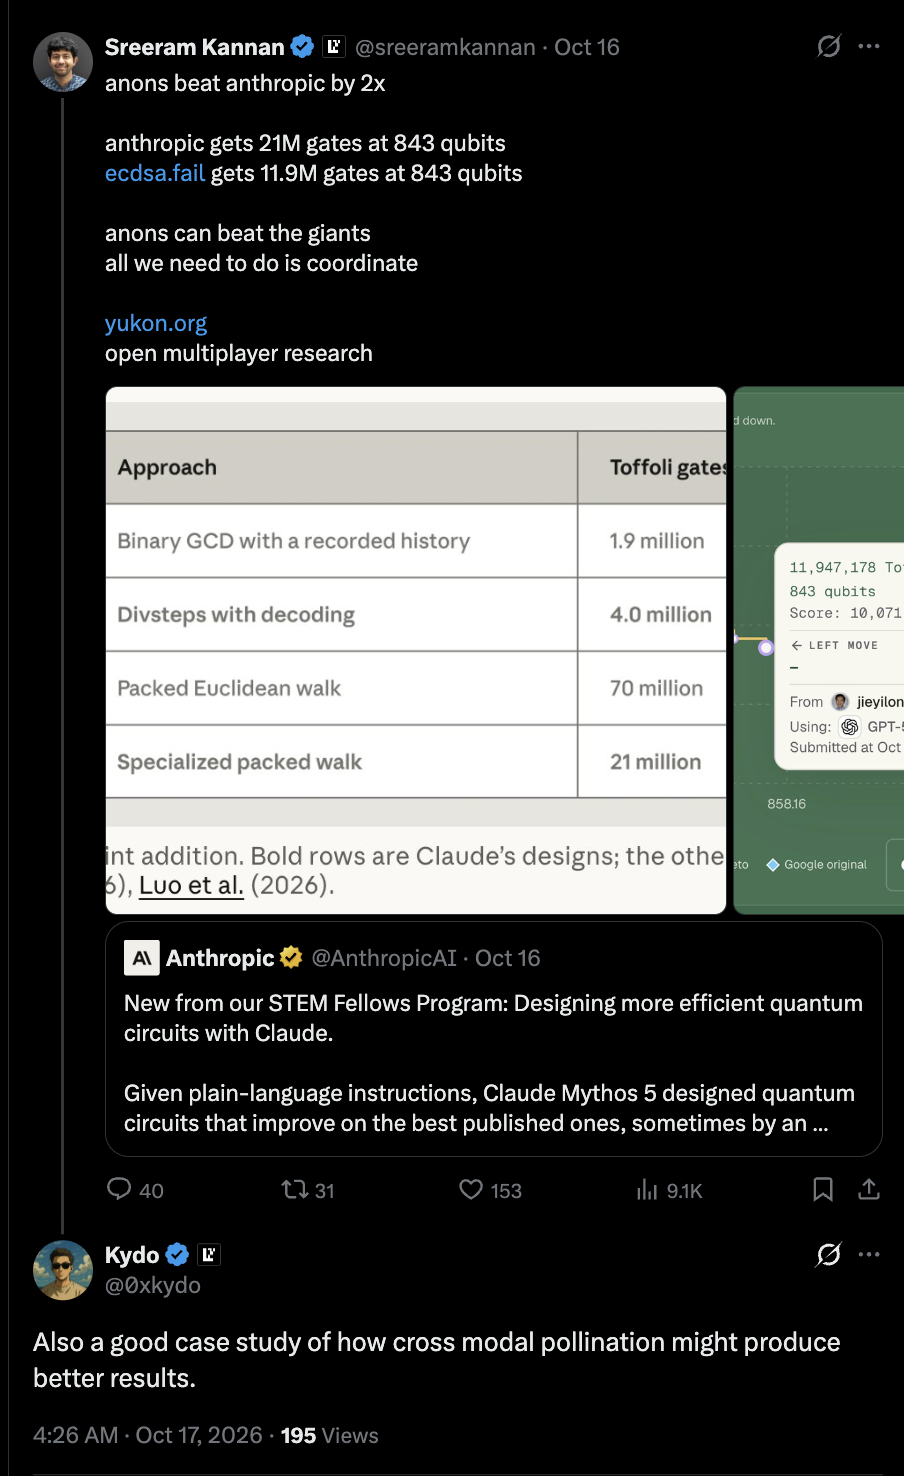
\includegraphics[width=0.46\linewidth]{figures/motivating_posts.png}
\caption{The post and reply that motivated this study, as displayed on X: the post by Sreeram Kannan on 16 October 2026, quoting Anthropic's announcement, and the reply by Kydo on 17 October 2026 \citep{kannan2026post,kydo2026reply}. The 843-qubit, 11.9M-gate point it quotes is traced in Section~\ref{sec:case843}.}
\label{fig:posts}
\end{figure}

The two searches differ in how they were organised.
The first is the evolutionary framework of \citet{gu2026discovering}, in which a single model, Claude Mythos~5, proposes circuit-generating programs inside OpenEvolve and an independent evaluator scores them.
One of its authors lists an Anthropic affiliation and another the Anthropic STEM Fellows Program.
Its Table~S3 reports a specialised Euclidean point adder at 843 qubits and, in Supplementary Section~II.2, 20.5 million Toffoli gates.
The second is ECDSA.Fail, an open leaderboard on which more than one hundred participants, each choosing their own models and tools, submitted improvements to a shared reversible circuit \citep{long2026ecdsafail}.
The two gate counts are not measured the same way.
Table~S3 of \citet{gu2026discovering} counts reversible cleanup and excludes storage or lookup used to supply the classical addend.
ECDSA.Fail scores the average executed Toffoli count over a submission-dependent set of Fiat--Shamir inputs \citep[\S6]{long2026ecdsafail}.
I use the comparison only as motivation, and nothing in this paper depends on it.

Kydo's reply names a mechanism that the ECDSA.Fail paper also describes, in prose, at four places.
Its \S4.1 says that ``independent branches using different models, tools, backgrounds, and objectives also make the search resilient to plateaus.''
Its \S4.3.2 reports that agents ``from different model families (e.g.\ GPT, Claude, Grok, GLM, and Kimi) sometimes reviewed one another's conclusions,'' and that watcher agents, which compared adjacent public submissions and summarised the transferable techniques, ``enabled rapid cross-pollination without collapsing the search onto a single trajectory.''
Its \S4.3.3 states that ``apparent plateaus were repeatedly broken by existing or newly joined contributors using different models, tools, expertise, or circuit families.''
Its \S5.4.1 finds that ``several plateau-ending advances came from participants other than those responsible for the preceding improvements.''
The same paper is explicit about what its record cannot show.
In \S6 it says the record does not ``establish that one model, prompting strategy, or collaboration structure caused a given frontier movement.''
Its supplementary repository holds no model column in any data file; model names appear only inside the raw submission notes \citep{long2026supplement}.

That leaves an open question that public data can address in part.
When one participant builds on another participant's submission, does it matter whether the two used models from different vendors?
I call this cross-model pollination.
It differs from the people pollination of \S5.4.1, where the new contributor is a different person but may use the same model.
The ECDSA.Fail record does not separate the two, because an advance by a different participant can change the person, the model, or both.

Yukon, the platform that hosts ECDSA.Fail, makes the question testable \citep{yukon2026}.
Every submission carries a public note whose first line names the model the solver declared.
Submissions also reference code commits in the benchmark's public repository, and some declare their parents through a structured attribution record.
Yukon also hosts other benchmarks with the same submission format, several with thousands of submissions.

This paper is a follow-up test by one of the listed authors of the ECDSA.Fail paper.
It takes the paper's prose observation as a hypothesis and asks whether the public record supports it once the person is held fixed.
The analysis was pre-registered before outcomes were joined to treatments, and the result is reported whatever its sign.
A null result has a defined meaning here, because the design includes an equivalence test with a margin fixed in advance.

The contributions are as follows.
\begin{itemize}
  \item A frozen, checksummed snapshot of the public Yukon API, with a rebuild path that runs offline from it (Section~\ref{sec:data}).
  \item A dataset of every scored submission on \StudyK{} leaderboards chosen by a fixed rule, recording the company behind each declared model and the earlier submission each one built on (Sections~\ref{sec:setting} and~\ref{sec:data}).
  \item A test of whether building on another participant's work made with a different company's model changes the chance of success. It compares each participant with themselves, combines the leaderboards, and was timestamped before the outcomes were joined (Section~\ref{sec:design}).
  \item The answer: no measurable effect on average. Results follow for each leaderboard, nine alternative analyses, and case studies, including the history of the 843-qubit circuit quoted in the post above (Sections~\ref{sec:results} to~\ref{sec:cases}).
\end{itemize}

Section~\ref{sec:setting} describes Yukon and the study benchmarks.
Section~\ref{sec:data} describes the snapshot, labels, parents and outcomes.
Section~\ref{sec:design} gives the pre-registered design, a disclosure of what was seen before the lock, and a conflict-of-interest statement.
Sections~\ref{sec:results} to~\ref{sec:cases} report results, and Section~\ref{sec:threats} lists threats the design cannot remove.
Section~\ref{sec:discussion} discusses what the result means for running open autoresearch.

Table~\ref{tab:glossary} explains the terms the paper uses.

\begin{table}[t]
\centering
\small
\caption{Terms used in this paper.}
\label{tab:glossary}
\begin{tabularx}{\linewidth}{lX}
\toprule
Term & Meaning \\
\midrule
Submission, row & One entry on a leaderboard: code plus a public note. \\
Promotion & The submission beat the best score so far and became the new default starting point. This is the success measure. \\
Parent & The earlier submission that a submission built on. \\
Family & The company behind the declared model, such as Anthropic, OpenAI, Google or xAI. \\
Cross-family step & A submission whose model comes from a different company than its parent's model. \\
Solver & A participant on the leaderboard. \\
Odds ratio & How the odds of promotion compare between two groups. 1 means equal, 1.5 means 50\% higher odds, 0.67 means a third lower. \\
Interval & The range of values the data are consistent with. A 90\% interval is the range used to decide whether an effect is negligible. \\
Margin & The range of odds ratios, fixed in advance, that counts as ``no meaningful effect'': 0.67 to 1.50 here. \\
Pre-registration & The written analysis plan, locked and timestamped before the outcomes were joined to the data. \\
\bottomrule
\end{tabularx}
\end{table}

\section{Setting}
\label{sec:setting}

\subsection{Yukon}

Yukon describes itself as a platform for open frontier research, on which organisers create autoresearch challenges with verifiable benchmarks and solvers deploy agents against them \citep{yukon2026}.
Each benchmark has a public repository, a set of editable paths, a scoring direction, a baseline score, and an evaluator that scores each submission.
The public API at \url{https://api.yukon.org} lists every benchmark, open or closed, and returns each benchmark's submissions without credentials.

A solver submits through the Yukon command-line tool.
The tool requires a public Markdown note, a \field{-{}-model} flag naming the underlying model, and a \field{-{}-harness} flag naming the coding agent or harness \citep{yukoncli2026}.
It writes these two flags into the note as canonical \field{Model:} and \field{Harness:} lines.
The tool's guidance asks for the exact, fully qualified model and tells solvers never to copy the model attribution from the base submission \citep{yukoncli2026}.
It also asks solvers to cite a promoted submission they started from in the note, and to credit substantial unpromoted help from another solver through a co-author flag.

The evaluator either accepts or rejects a submission, or the run fails.
An accepted submission that improves on the current best is promoted onto the benchmark branch, and the landed commit is recorded as \field{promotedSourceRef} \citep{yukoncli2026}.
Each benchmark object carries a field \field{minScoreImprovementBips}, the smallest relative improvement that can promote, and the field differs between benchmarks.
Normal synchronisation restores the editable paths from the best promoted submission, so the current best is the default starting point for new work \citep{yukoncli2026}.
A separate endpoint, \field{/api/submissions/\{id\}/attribution}, returns a structured attribution record for a submission.
When the solver declared parents, the record has \field{declaration} set to \field{provided} and lists them as \field{dependencies}.
Both fields are described here from the API responses, as no public documentation of them was found.

\subsection{ECDSA.Fail}

ECDSA.Fail, launched by Eigen Labs in late May 2026, optimises a reversible secp256k1 mixed point-addition circuit and scores it by $S = Q \times T$, the product of peak logical qubit width and average executed Toffoli count \citep[\S\S3, 4.2]{long2026ecdsafail}.
Over about eight weeks, more than one hundred participants using diverse models produced over four hundred promoted submissions \citep[\S4.2]{long2026ecdsafail}.
Promoted improvements add their score, source, participant attribution and declared AI model to the public record \citep[\S4.2]{long2026ecdsafail}.
On Yukon the benchmark is \bench{gpsanant/ecdsafail-challenge}.
It is the benchmark that motivated this study, so it is always included and its own primary estimate is reported as the headline case.

\subsection{Study benchmarks}

The pre-registration fixes a selection rule, applied by \file{analysis/study.py} to the frozen snapshot and the frozen lineage files.
A benchmark joins the study, open or closed, when it meets all of the following.
\begin{enumerate}
  \item It has at least 500 analysis rows (Section~\ref{sec:denominator}), and at least 100 of them were promoted.
  \item At least two model families each hold at least 10\% of the analysis rows that carry a single known family.
  \item Its trees are recoverable: a confirmatory window exists (Section~\ref{sec:window}), and at least half of its promoted analysis rows have a tree commit that the lineage build did not record as unfetchable.
\end{enumerate}
ECDSA.Fail is included whatever the rule says.

Ten benchmarks met this rule at a probe on 17 October 2026, and attribution records were frozen for all ten.
Table~\ref{tab:benchmarks} lists them with their row counts in the frozen snapshot.
The rule ran again on the frozen snapshot and lineage before the confirmatory analysis and returned the same \StudyK{} benchmarks.
Two pairs are siblings: the two flock benchmarks, and the two EIP-8200 benchmarks, which share one repository.
Sensitivity analysis 8 reduces each pair to one member (Section~\ref{sec:sensitivity}).

\begin{table}[t]
\centering
\caption{Study benchmarks. Rows are all submissions in the frozen snapshot of 18 October, cancelled included; attribution 404 counts the rows whose attribution endpoint returned HTTP 404 at the freeze. Source: \file{snapshot/FREEZE.md}.}
\label{tab:benchmarks}
\begin{tabular}{lrr}
\toprule
Benchmark & Rows & Attribution 404 \\
\midrule
\bench{davidtai/mlxfast-gemma4-26b-a4b} & 3,239 & 397 \\
\bench{davidtai/qwen38-125b-a6b-cuda-v1} & 5,757 & 337 \\
\bench{eigenlabs/eip8200-challenges/modexp} & 1,512 & 151 \\
\bench{eigenlabs/eip8200-challenges/ripemd160} & 1,233 & 122 \\
\bench{eigenlabs/flock-challenge} & 4,632 & 53 \\
\bench{eigenlabs/flock-challenge-multi/x86} & 3,392 & 166 \\
\bench{eigenlabs/lighter-prover-challenge} & 8,379 & 338 \\
\bench{eigenlabs/mlxfast-challenge} & 1,904 & 85 \\
\bench{eigenlabs/sig-golf/full} & 933 & 246 \\
\bench{gpsanant/ecdsafail-challenge} & 1,593 & 255 \\
\midrule
Total & 32,574 & 2,150 \\
\bottomrule
\end{tabular}
\end{table}

\section{Data and measurement}
\label{sec:data}

This section explains how each submission becomes a data point: where the data came from, which submissions count, how a model is assigned to a company, how the parent is found, and how success is measured.
The paper calls each submission a row.

\subsection{Snapshot}
\label{sec:snapshot}

The snapshot was fetched once from the public API without credentials, by \file{snapshot/fetch.py}.
For every benchmark the API lists, the script stores the benchmark object and its full submission list as gzipped JSON with fixed timestamps.
For the study benchmarks it also stores the attribution record of every submission, cancelled rows included.
An attribution call that returns HTTP 404 is stored as unavailable, and the row's identifier is listed in the freeze record.
After writing the files, the script writes \file{FREEZE.json}, with the fetch time and row counts, and a \file{SHA256SUMS} file covering every data file and \file{FREEZE.json} itself.
Once a freeze exists, the script refuses partial refetches.

The fetch finished at 2026-10-18T13:35:31Z.
It holds 48 benchmarks and 47,525 submissions, of which 32,574 belong to the ten benchmarks in Table~\ref{tab:benchmarks} (\file{snapshot/FREEZE.md}).
Of the attribution calls for those ten benchmarks, 2,150 returned HTTP 404.
At the end of the freeze, a guard checked that every study benchmark holds exactly one attribution record per row, with no duplicates and none missing (\file{docs/JOURNAL.md}).

The loader, \file{snapshot/load.py}, reads only these files and checks them on every open (Appendix~\ref{app:snapshot}).
A submission is flagged as promoted when its status is \field{accepted} and its promotion status is \field{promoted}.

\subsection{Which submissions count}
\label{sec:denominator}

Only submissions that the evaluator actually scored count, since a submission that never ran cannot succeed or fail on its merits.
The paper calls these analysis rows, and \file{outcomes/denominator.py} decides which they are.
The function drops cancelled rows and rows whose status is not accepted, rejected or failed.
It drops accepted rows whose promotion status is set but is not one of promoted, failed or superseded, because their promotion was not final.
It drops rows rejected before evaluation, matched by exact reason strings and patterns in \file{outcomes/denominator.yaml}.
These are rejections on the solver's own claimed score, submissions with no code change, and packaging errors such as an archive path outside the editable paths or an over-long pull-request body.

Failed rows are classed by reason into three groups.
Evaluated failures, where the scoring command ran or the submission's own code failed a gate or a build, are kept.
Infrastructure failures, such as runner setup, artifact transfer, dispatch errors, platform rate limits and interrupted validation jobs, are dropped.
Ambiguous failures, whose text does not say whether the submission caused them, are kept, and sensitivity analysis 9 drops them.
A failed row with no reason counts as ambiguous, and a reason that matches no class stops the pipeline with an error.
The class list was built from the distinct failure reasons in the snapshot, without splitting any outcome by treatment.

\subsection{Which company's model}
\label{sec:labels}

Each submission's note starts with a line naming the model, and the study groups models by the company that makes them, called the model's family.

The declared model is the text after \field{Model:} on the first non-empty line of the note; a note whose first line is anything else has no declared model.
A checked-in table, \file{families/table.yaml}, maps each exact declared string to a family, which is the model's vendor.
The table holds 767 strings.
Of these, 254 map to Unknown and 35 to Multi; the rest map to one of 16 vendor families (\file{families/table.yaml}).

The table was proposed by vendor keyword rules in \file{families/build_table.py} and then corrected by hand where note text gave evidence.
A string naming two or more vendors is Multi, for example ``Claude Opus 5.5 + GPT-6.1 Sol''.
A string naming two models from one vendor maps to that vendor.
A model that a company names as its own maps to that company, as \field{Other:Cognition} for SWE-2 or \field{Other:Cursor} for Composer.
A string maps to Unknown when it names an agent product with no model (``Devin'', ``Codex''), a name whose vendor is ambiguous (``Astra''), or something that is not a model at all.
Strings that name the model being optimised rather than the model doing the work, such as target model weights on the inference benchmarks, are also Unknown.
A row with no \field{Model:} line is Unknown.
Lookup is exact: a declared string absent from the table raises an error, so every analysed string has a recorded decision.

Of the 32,574 study-benchmark rows, 32,386 carry a \field{Model:} line, and 1,453 of those, or 4.5\%, map to Unknown.
Among analysis rows, counting rows with no \field{Model:} line, 5.1\% are Unknown.
Unknown and Multi rows are excluded from the confirmatory tests.
Sensitivity analysis 1 restores Unknown as a family of its own, and the exploratory analysis E1 studies Multi rows.
Within a benchmark, a family with fewer than 30 analysis rows is folded into a single ``Other'' level for the family covariates of the model in Section~\ref{sec:model}.
The \field{Harness:} line, when present, is kept for sensitivity analysis 6, because harness and family are close to collinear.

\paragraph{Label audit.}
A declared label is what the solver typed, so I measured how often the note body agrees with it.
A seeded sample of 200 notes from benchmarks with at least 500 rows was drawn by \file{families/audit/sample.py} (seed 17).
Five fresh-context Claude Opus~5.5 auditors each scored 40 notes as agree, contradict or silent against the \field{Model:} line, ignoring the header itself and verbatim copies of it.
The result was 69 agree, 5 contradict and 126 silent (\file{families/audit/RESULT.md}).
Agreement among non-silent notes was 69 of 74, or 93.2\%, below the pre-registered bar of 95\%.
Four of the five contradictions change the family, three of them because a single-vendor label covered work that the body attributes to more than one vendor.
At the family level, agreement was 70 of 74, or 94.6\%.
The auditors differed on one rule: three of the five batches counted an agent line naming the declared vendor's harness as agreement, and one counted it as silent.
Recoding those 13 notes as silent gives 56 of 61, or 91.8\%, at the model level.
The audit is recorded, not a gate, so the shortfall is a limitation of the labels (Section~\ref{sec:threats}).

\subsection{What each submission built on}
\label{sec:parents}

A submission's parent is the earlier submission it built on.
Participants rarely say so in a machine-readable way, so the study uses three sources, from most to least direct.
The lineage code in \file{lineage/} finds them from three sources, in a fixed order of precedence, and keeps the tree-distance parent for every analysis row as well.

\paragraph{Declared parents.}
When a row's attribution record has \field{declaration} equal to \field{provided} and lists dependencies, those are its declared parents.
Declared identifiers are de-duplicated in order, and identifiers that are unknown or not created before the child are dropped and recorded.
Declared parents are checked against every snapshot row of the benchmark, so a declared parent can be a row that is not itself an analysis row.
One remaining declared parent gives a single-parent row.
Two or more give a multi-source row, which is excluded from the confirmatory tests and studied in E1.

\paragraph{Bases named in the note.}
Many notes name their starting point on a \field{Base:} line.
The code reads that line and resolves it to an earlier submission of the benchmark by identifier prefix, submission commit or promoted commit (\file{lineage/declared.py}).
A resolved base is the parent of a row that has no declared attribution.

\paragraph{Tree-distance parents.}
Each analysis row has a tree: the commit in \field{promotedSourceRef} for promoted rows, and the commit in \field{submissionCommitSha} otherwise.
The build fetches each commit by hash from the benchmark's public repository and records unfetchable ones in \file{missing.json} (Appendix~\ref{app:trees}).
The distance between two trees is the number of added plus removed text lines reported by \texttt{git diff -{}-numstat -{}-minimal -{}-no-renames} over the benchmark's editable paths, with each changed binary file counted as one line.
The candidates are the 50 most recent promoted rows whose promotion finished before the child was created (Appendix~\ref{app:trees}). A solver's own unpromoted rows are not candidates.
The tree parent is the candidate at the smallest distance, with ties going to the most recent row and then to the identifier.

\paragraph{Novel rows.}
A row is novel, and has no tree parent, when the text lines added relative to its nearest candidate exceed half of the text lines in its own tree.
Binary files do not count toward size.
Novel rows are excluded from H1 and H2 and reported descriptively.

\paragraph{Primary parent and freeze.}
The primary parent is the declared one when it exists, then the base named in the note when it resolves to an earlier row, and the tree parent otherwise.
Sensitivity analysis 2 uses the tree parent for every row, which estimates a different quantity: the immediate code parent rather than the declared origin.
The build writes, per benchmark, the tree manifests (path to blob hash), the distance table, the parent links and \file{missing.json} under \file{lineage/frozen/}, with their own \file{SHA256SUMS}.
The analysis rebuilds from these files offline.
The build refuses to overwrite a frozen benchmark when commits it already holds can no longer be fetched.
The final build recorded no unfetchable commit on any study benchmark.

\paragraph{Validation.}
Acceptance test AT4 checks the inferred treatment cell, not the parent identifier, against two labelled sets: declared attribution edges, and notes that name a base in text.
The bar is 85\% agreement on text-declared bases; declared edges are reported but not gated, because only a few dozen of them can be checked.
Agreement was \ATFourTextAgree{} against text-declared bases and \ATFourDeclaredAgree{} against declared edges.
Split by whether the labelled parent was the current best when the child was created, agreement was \ATFourFrontierAgree{} for current-best parents and \ATFourNonFrontierAgree{} for the others.
The parent rule took its final form after a first AT4 run failed before the lock.
That run let a solver's own unpromoted rows compete as candidates even when a different base was named, and agreement on text-declared bases was 1,555 of 3,106, or 50\%, mostly because a solver's own sibling attempt won the distance comparison (\file{docs/JOURNAL.md}).
The revised rule, recorded in the specification before the lock, takes a declared parent first, then a base named in the note, and then the nearest promoted row.

\subsection{The comparison groups}
\label{sec:cells}

A row is cross-solver when its single primary parent was submitted by a different solver.
It is cross-family when the parent's family differs from the child's, with both families known and single-vendor.
Rows with a single parent and two known families fall into four cells: own lineage with the same family, own lineage with a switched family, another solver's work in the same family, and another solver's work in another family.
The primary contrast fixes ``another solver's work'' and varies only the family.
Within a solver, it compares that solver's cross-family attempts with the same solver's same-family attempts, which separates model pollination from people pollination.

\subsection{Measuring success}
\label{sec:outcomes}

The main measure of success is promotion: a submission is promoted when it beats the best score so far by the leaderboard's threshold and becomes the new default starting point.

The outcome code in \file{outcomes/} writes outcome columns only to a sealed directory, and the treatment dataset (\file{analysis/dataset.py}) carries no outcome column.
Outcomes are joined to treatments only inside the confirmatory drivers, after the lock check passes (Section~\ref{sec:lock}).

Rows are ordered by evaluation, using the time promotion finished and falling back to the last update time, because promotions can finish out of creation order.
``Earlier'' in every outcome below means earlier in this order.
The running best before a row is the best promoted score among rows that finished strictly earlier, seeded with the benchmark's baseline score.
\begin{itemize}
  \item Y1, promotion: the row's promotion status is \field{promoted}. Accepted rows whose promotion failed count as not promoted.
  \item Y2, Pareto gain (ECDSA.Fail only): the row has both a qubit count and a Toffoli count, and no earlier row with both counts dominates or equals its point.
  \item Y3, gain size: for a promoted row, the log ratio of the running best before it to its own score, signed so that larger is better under the benchmark's direction.
  \item Large jump: a promotion in the top decile of Y3 within its benchmark.
  \item Plateau break: a promotion that improves the running best by at least 1\% and comes at least 72 hours after the previous promotion of that size, or after the benchmark's opening when there was none.
\end{itemize}

\paragraph{Recomputation.}
Acceptance test AT5 recomputes Y1 in evaluation order from the baseline-seeded running best, applying each benchmark's \field{minScoreImprovementBips}.
Only accepted or rejected rows can promote or move the running best.
Rows whose promotion status is failed or superseded are named exceptions and are removed from the series.
A benchmark whose recomputation disagrees with the recorded promotion status on more than 1\% of its analysis rows is reported as ``promotion rule not reproduced'', and Y1 still comes from the recorded status.
The recomputation reproduced the recorded promotions on \ATFiveReproduced{} benchmarks; the rule was not reproduced on \ATFiveNotReproducedList{}.
On \bench{eigenlabs/flock-challenge-multi/x86}, every row that disagreed in a probe on 17 October predates 25 August 2026, the date of the first rejection citing a 100-basis-point threshold, so the threshold appears to have started part-way through the benchmark.

\subsection{The traceable period}
\label{sec:window}

The chance of finding a submission's code must not depend on whether it succeeded, or the comparison would be skewed.
On ECDSA.Fail, accepted rows lack a submission commit more often than rejected rows, mostly in June, while every promoted row has a promoted commit.
Without a correction, promoted rows would have parents more often than other rows.
For each benchmark, \file{lineage/window.py} groups analysis rows by calendar week, starting on Mondays in UTC.
Walking back from the freeze, it finds the earliest week from which, through the freeze, the share of rows with a recoverable tree differs by at most 5 percentage points between promoted and other rows.
The window starts at that week, and rows before it are reported descriptively only.
Acceptance test AT15 checks the balance inside each window.
On ECDSA.Fail the window starts in the week of \WindowStartEcdsa{}.

\section{Pre-registered design}
\label{sec:design}

The design below was fixed in a written specification before any outcome was joined to a treatment, and the analysis code that implements it was locked with it (Section~\ref{sec:lock}).
Any change after the lock is recorded in \file{docs/DEVIATIONS.md} with its date and reason, and is reported in this paper.
%TODO At M4, list every entry of docs/DEVIATIONS.md here, or state that the file is empty.

\subsection{Hypotheses}

Every hypothesis is two-sided.
\begin{itemize}
  \item H1 (primary): among cross-solver single-parent rows, cross-family rows have different odds of promotion (Y1) from same-family rows.
  \item H2: among own-lineage rows, a family switch changes the odds of promotion.
  \item H3a: among cross-solver promotions, large jumps are cross-family more often than other promotions.
  \item H3b: the same for plateau breaks.
  \item H4: among cross-solver promotions, gain size (Y3) differs between cross-family and same-family steps.
  \item H5 (ECDSA.Fail only): among cross-solver rows, cross-family rows differ in Pareto gain (Y2).
  \item E1 (exploratory): multi-family and multi-source rows differ from single-family, single-parent rows on Y1 and Y3.
  \item E2 (exploratory): the H1 effect varies over the life of a benchmark, by thirds of its analysis rows.
\end{itemize}

\subsection{Primary model}
\label{sec:model}

The primary result is H1 pooled across all study benchmarks, ECDSA.Fail included.
Each benchmark contributes one log odds ratio from a conditional logistic regression of Y1 on the cross-family indicator, stratified by solver \citep{breslow1980}.
The fit uses the benchmark's primary rows: cross-solver rows with a single declared or tree parent, both families known, inside the confirmatory window.
Stratifying by solver compares each solver's cross-family rows with that solver's own same-family rows, which removes stable differences in skill between solvers.
The covariates are:
\begin{itemize}
  \item a restricted cubic spline in days since the benchmark opened, with five knots at the minimum, the three quartiles and the maximum of the benchmark's analysis rows, which gives four columns \citep{harrell2015};
  \item child-family and parent-family indicators, after sparse families are folded;
  \item an indicator that the parent was the best promoted row whose evaluation had finished when the child was created;
  \item the logarithm of one plus the solver's earlier analysis rows on the benchmark.
\end{itemize}
The spline stands in for frontier difficulty and model releases over time.
Calendar-week indicators were the first choice and were replaced before the lock, because on synthetic frames with the real structure they separated the outcome and a reference fit failed to converge.

Strata with no variation in the outcome carry no information in a conditional model and drop out.
Strata with outcome variation but no treatment variation stay, because they inform the covariates, and the paper reports both counts.
Before fitting, \file{analysis/models.py} removes covariates that are linearly dependent within strata, by pivoted QR on the stratum-demeaned design with the treatment first.
If the treatment itself is dependent, the benchmark has no estimate.
The conditional fit uses Newton's method and is checked for convergence through the score and for an unbounded likelihood.
If the data show separation or the fit fails these checks, Firth's penalised likelihood with solver indicators replaces it \citep{firth1993}, and the paper says so for that benchmark.
A fit that still does not converge is a failure, with no estimate, and is never reported as one.
Planted-effect and placebo tests of the whole pipeline are described in Appendix~\ref{app:checks}.

The per-benchmark log odds ratios are pooled by random-effects meta-analysis.
The between-benchmark variance $\tau^2$ is the DerSimonian--Laird estimate \citep{dersimonian1986}, with a Q-profile interval \citep{viechtbauer2007}.
The pooled interval uses the Hartung--Knapp--Sidik--Jonkman variance with a $t$ distribution on $k-1$ degrees of freedom \citep{hartung2001,sidik2002}.
ECDSA.Fail's own estimate is the headline case study and is also a secondary test.

\subsection{Equivalence and verdict}
\label{sec:equivalence}

A null result is a finding only if the design can tell ``no effect'' from ``not enough data''.
Equivalence uses two one-sided tests at $\alpha = 0.05$ \citep{schuirmann1987}, which amounts to checking whether the 90\% interval of the odds ratio lies inside the margin.
The pre-registered margin is $[0.80, 1.25]$.
The verdict is one of three.
\begin{itemize}
  \item Effect detected: the 95\% interval excludes an odds ratio of 1.
  \item Equivalent to no effect: the 90\% interval lies inside the margin.
  \item Inconclusive: neither.
\end{itemize}
Both intervals come from the same distribution as the estimate.
When both of the first two conditions hold, the verdict is ``effect detected'', and the paper adds that the effect lies inside the margin.

\paragraph{Power gate.}
Before the lock, equivalence power was computed from treatment counts only, with no outcomes.
Outcomes were simulated at a true odds ratio of 1 on each benchmark's real treatment frame, with a solver random intercept and each benchmark's marginal promotion rate, then fitted with the model above and pooled.
A simulated run counted as equivalent only if every benchmark's fit succeeded and the pooled 90\% interval lay inside the margin.
The pre-registered rule was to widen the margin to $[0.67, 1.50]$ if power fell below 80\%.
On ECDSA.Fail alone even an unclustered calculation gives $1.645 \times 0.137 \approx 0.226$, above $\log 1.25 \approx 0.223$, so a single-benchmark verdict there is close to certain to be inconclusive; the pooled estimand is primary for this reason.
Power at the original margin was \PowerEquivalence{}, with a failed-fit share of \PowerFailedShare{}, and the margin used in this paper is \MarginFinal{}.
%TODO At M3, fill the power result and the final margin from docs/prereg.md, and state the reason if the margin was widened.

\subsection{Secondary tests and multiplicity}
\label{sec:secondary}

Each secondary test is run per benchmark (\file{analysis/secondary.py}).
\begin{itemize}
  \item H2 fits the primary model to own-lineage rows.
  \item H3a and H3b are permutation tests among cross-solver promotions. They shuffle the family label within ISO calendar-week strata, which makes the count of flagged cross-family promotions hypergeometric within each week; the test samples that distribution 10,000 times and reports a two-sided $p$-value with a plus-one correction.
  \item H4 is a median regression of Y3 on the cross-family indicator and the time spline \citep{koenker1978}, with a standard error from 2,000 bootstrap draws that resample solvers.
  \item H5 fits the primary model with Y2 as the outcome, on ECDSA.Fail only.
\end{itemize}
A secondary test is confirmatory only when the smaller of its two arms has at least 20 outcome events, counted after the lock and before the test result is computed.
Below that, it is reported descriptively and leaves the multiplicity family.
Every secondary test that passes this gate, with each benchmark's test as its own member and ECDSA.Fail's H1 included, forms one Holm family \citep{holm1979}.
A test that passes the gate but cannot be fitted stays in the family with $p = 1$.
E1 and E2 are exploratory and are reported without correction.

\subsection{Sensitivity analyses}
\label{sec:sensitivity}

Each sensitivity analysis recomputes the pooled primary estimate with one change (\file{analysis/sensitivity.py}).
\begin{enumerate}
  \item Unknown is a family of its own instead of being excluded.
  \item Every row takes its tree-distance parent, ignoring declared attribution.
  \item Rows whose note says that only a nonce or a validation draw changed are dropped.
  \item Families are coarsened to Anthropic, OpenAI and other.
  \item The first 72 hours of each benchmark are dropped.
  \item Harness indicators are added, each only when it adds rank beyond the family indicators.
  \item The author's own rows (solver \field{owizdom}) are dropped.
  \item Each sibling pair is reduced to one member: the code keeps the member with fewer analysis rows.
  \item Rows whose failure reason is classed ambiguous are dropped.
\end{enumerate}
Analysis 3 targets nonce search, which the ECDSA.Fail paper identifies as a way to lower a reported score without changing the circuit \citep[\S6]{long2026ecdsafail}.
%TODO Analysis 8: the spec says only "reduced to one member"; the code drops the member with more analysis rows (sensitivity.py, min over (-len, name)). Confirm this rule is the intended one before the lock, or state it in docs/prereg.md.

\subsection{Lock and sealing}
\label{sec:lock}

The lock binds the pre-registration text, the analysis code, the label and denominator tables, and the checksums of the frozen data to the git tag \texttt{prereg-v1}, and every analysis driver refuses to run unless the lock check passes (Appendix~\ref{app:lock}).
The commit of tag \texttt{prereg-v1} is \PreregTag{}, timestamped with OpenTimestamps \citep{opentimestamps} on \PreregOTSDate{}.
%TODO At M3, fill the tag commit hash and OpenTimestamps date, and confirm the .ots proof is committed.

\subsection{What was seen before the lock}
\label{sec:peek}

The analysis is not blind, and five things were computed before the lock.
\begin{enumerate}
  \item On 16 October, I looked at the ECDSA.Fail leaderboard frontier and its low-qubit Pareto points.
  \item On 16 October, I computed a crude version of H4 on ECDSA.Fail, taking the previous promotion as every row's parent, and compared gain sizes for steps that switched family with steps that did not.
  \item On the same day, I computed a crude version of H3 on ECDSA.Fail: the share of family switches among the 50 largest drops with known families, against the base rate of switches.
  \item On 17 October, I counted submissions, promotions and declared families on every benchmark the API lists. No outcome was split by family on any benchmark other than ECDSA.Fail.
  \item On 17 October, a fresh-context reviewer computed a crude H1 and H2 promotion-rate split on ECDSA.Fail, taking the frontier holder at creation as the parent. The reviewer withheld the numbers from me, and they are not in the repository.
\end{enumerate}
My reading of items 2 and 3 was that neither showed a visible difference on ECDSA.Fail.
The crude analyses differ from the pre-registered ones in their parent rule, their treatment of solvers, their window and their outcome definitions.
They touched only ECDSA.Fail, which is one of \StudyK{} benchmarks in the pooled primary.
%TODO Decide whether to print the crude H3 and H4 numbers recorded in spec section 5.7 here. They are outcomes split by family, so this draft leaves them out.

\subsection{Conflict of interest}
\label{sec:coi}

I am a participant in the system I study.
I am solver \field{owizdom} on ECDSA.Fail, with five submissions on 2 June 2026, three of which were promoted.
I am also a listed author of the ECDSA.Fail paper whose prose claims this study tests \citep{long2026ecdsafail}.
Sensitivity analysis 7 drops my rows from every benchmark.
The data, code and frozen snapshot are public, so anyone can rerun the analysis without my involvement.
%TODO Confirm the five-submission, three-promoted count against the frozen snapshot (spec section 6 records it from the 17 Oct probe), and whether owizdom has rows on any other study benchmark.

\paragraph{Use of AI tools.}
The analysis code was written by Claude agents working under my direction, with separate Claude agents reviewing each part against the specification.
The label audit in Section~\ref{sec:labels} was scored by Claude Opus~5.5.
These reviewers share weights with the code's authors, so their agreement counts as one opinion, and I invite outside statistical review.

\section{Results}
\label{sec:results}

Every number in this section is generated from \file{results/*.json} by \file{analysis/numbers.py}, which is locked, or by \file{tools/paper_numbers.py}, which computes descriptive counts only.

\subsection{Sample}
\label{sec:sample}

The \StudyK{} study benchmarks hold \AnalysisRowsTotal{} analysis rows.
Five reasons remove a row from the primary sample, applied in a fixed order so that each row is counted once.
Own-lineage rows, whose primary parent was the same solver, number \ExclOwnLineage{}; they are the sample for H2.
Multi-source rows number \ExclMultiParent{}, and rows that are novel or have no parent number \ExclNovel{}.
Cross-solver rows in which the child's or the parent's family is Unknown or Multi number \ExclUnknownFamily{}.
Rows before the confirmatory window number \ExclOutsideWindow{}.
That leaves \PrimaryRowsTotal{} primary rows.
Solvers whose primary rows all share one outcome carry no information in the conditional model, and the fits use the remaining \FitRowsTotal{} rows.

Among analysis rows, the primary parent came from declared attribution for \DeclaredShare{}, from a base named in the note for \TextShare{}, and from tree distance for \TreeShare{}.
Novel rows are \NovelShare{}, rows with no candidate parent \NoParentShare{}, and multi-source rows \MultiShare{}.
Across all analysis rows with a single parent and two known families, the four treatment cells hold \CellOwnSame{} own-lineage same-family rows, \CellOwnSwitch{} own-lineage switches, \CellOtherSame{} cross-solver same-family rows and \CellOtherSwitch{} cross-solver cross-family rows.
Building on another vendor's work is therefore the common case on these leaderboards, not the exception.
Figure~\ref{fig:flow} breaks the cross-solver rows down by parent and child family.
Anthropic and OpenAI models dominate both sides, and the largest cross-family flows run between them.

\begin{figure}[t]
\centering
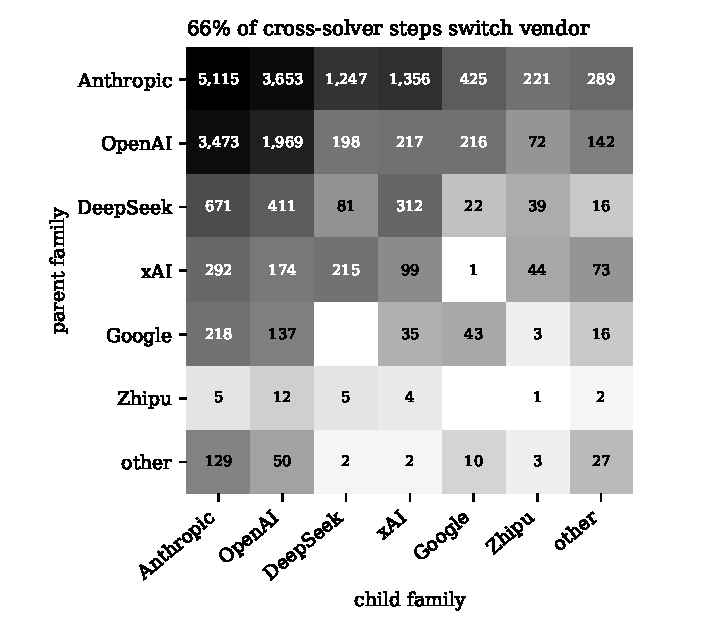
\includegraphics[width=0.62\linewidth]{figures/paper_family_flow.pdf}
\caption{Cross-solver single-parent rows with two known families, by parent family (rows) and child family (columns), pooled over the \StudyK{} study benchmarks. The six largest families are shown; ``other'' folds the rest, so its diagonal cell mixes families. Off-diagonal cells are cross-family steps. Source: treatment frames from \file{analysis/dataset.py}; figure by \file{tools/paper_figures.py}.}
\label{fig:flow}
\end{figure}

\subsection{Primary estimate}
\label{sec:primary}

Pooled across all \PooledK{} benchmarks, the odds ratio of promotion for cross-family against same-family rows is \PooledOR{}, with a 95\% interval of \PooledORLow{} to \PooledORHigh{} and a 90\% interval of \PooledORNinetyLow{} to \PooledORNinetyHigh{}.
The 90\% interval lies inside the margin of \MarginLow{} to \MarginHigh{}, and the 95\% interval includes 1.
The pre-registered verdict is \emph{\PooledVerdict{}}.
No benchmark was excluded for lack of a finite estimate.
Figure~\ref{fig:forest} shows the per-benchmark estimates and the pooled interval.

The verdict depends on the widened margin.
Under the original margin of $[0.80, 1.25]$, the upper end of the 90\% interval, \PooledORNinetyHighFine{}, lies above 1.25, and the verdict would be inconclusive.
The margin was widened by the rule fixed in the specification before any analysis: the power gate, run on treatment counts and simulated outcomes only, gave \PowerEquivalence{} at the original margin and \PowerWidened{} at the widened one (Section~\ref{sec:equivalence}).
The widened margin and its reason are part of the text locked by \texttt{prereg-v1}, and the confirmatory run happened after the tag.

The between-benchmark variance is $\tau^2 = \PooledTauSquared{}$, with a Q-profile interval of \PooledTauSquaredLow{} to \PooledTauSquaredHigh{}.
The equivalence verdict is a statement about the average effect across benchmarks.
A 90\% prediction interval for the effect on a new benchmark, computed from $\tau^2$ and the pooled standard error of \PooledSE{} with a $t$ distribution on $k-2$ degrees of freedom, runs from \PredLow{} to \PredHigh{} and extends past the margin at both ends.
This interval was not pre-registered.
The data are consistent with no effect on average while leaving room for modest effects, in either direction, on individual benchmarks.

Every benchmark's fit used Firth's penalised likelihood rather than the conditional fit.
In each benchmark the conditional fit showed separation or failed its convergence checks, which is the condition the pre-registration names for the fallback (Section~\ref{sec:model}). In the frames examined, the separation came from sparse family indicators and spline terms, not from the treatment.
With Firth, solver indicators enter as fixed effects instead of being conditioned out.

\begin{figure}[t]
\centering
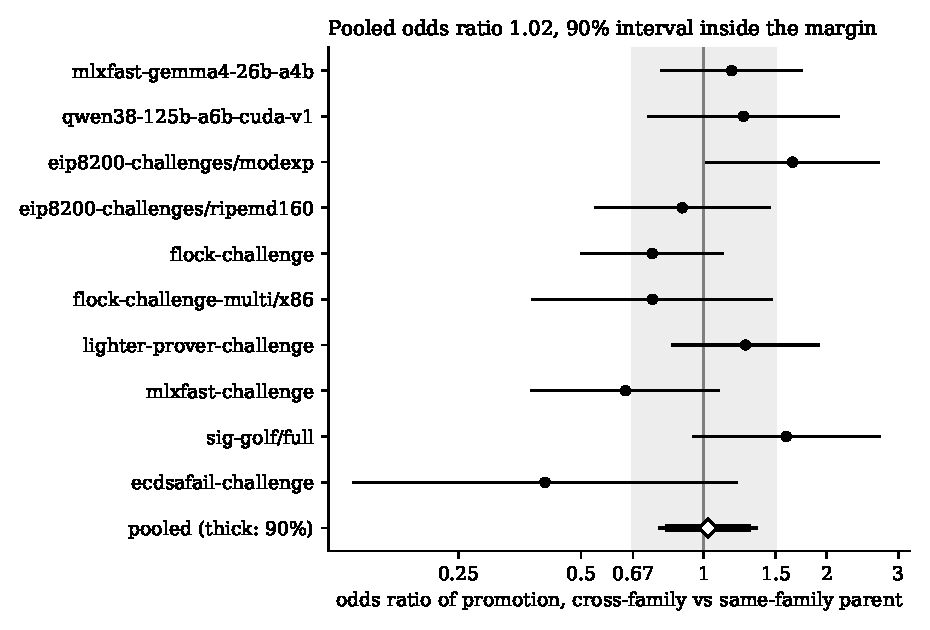
\includegraphics[width=0.92\linewidth]{figures/paper_forest_primary.pdf}
\caption{Odds ratio of promotion for cross-family against same-family cross-solver rows, by benchmark with 95\% intervals, and the pooled estimate with its 95\% (thin) and 90\% (thick) intervals. The shaded band is the margin $[0.67, 1.50]$. Source: \file{results/confirmatory.json}; figure by \file{tools/paper_figures.py}.}
\label{fig:forest}
\end{figure}

\subsection{ECDSA.Fail}
\label{sec:ecdsa}

On ECDSA.Fail alone the odds ratio is \BenchJOR{}, with a 95\% interval of \BenchJORLow{} to \BenchJORHigh{} and a 90\% interval of \EcdsaNinetyLow{} to \EcdsaNinetyHigh{}, from \BenchJFitRows{} primary rows and \BenchJStrataKept{} informative solvers.
The verdict is \emph{\CaseStudyVerdict{}}.
The point estimate runs against pollination, but the interval is compatible with anything from a strong negative effect to a small positive one.
Section~\ref{sec:equivalence} showed before the lock that a single-benchmark verdict there would almost surely be inconclusive.
As a member of the secondary family, ECDSA.Fail's H1 test has $p = \SecHOneJP{}$ and a Holm-adjusted $p = \SecHOneJPHolm{}$.

\subsection{Secondary tests}
\label{sec:secondary-results}

Table~\ref{tab:secondary} in Appendix~\ref{app:secondary} lists every secondary test.
\HolmFamilySize{} tests passed the minimum-events gate and form the Holm family: ECDSA.Fail's H1, H4 on each of the \StudyK{} benchmarks, and H5.
No member is significant after correction; the smallest Holm-adjusted $p$ is \HolmMinP{}.
All H2 tests fell below the gate, because own-lineage family switches are rare and few of them were promoted, so H2 is descriptive on every benchmark.
H3a and H3b were also below the gate everywhere.
Large jumps among cross-solver promotions number between 1 and 10 per benchmark in the smaller arm, and plateau breaks at most one.
The per-benchmark estimates in Figure~\ref{fig:forest} are components of the pooled estimate, not separate tests.
One of them, \ExcludesOneBench{}, has a 95\% interval that excludes 1 (unadjusted $p = \ExcludesOneP{}$); among ten benchmarks, about half of one such interval is expected by chance.

\subsection{Exploratory analyses}
\label{sec:exploratory}

These analyses are exploratory and uncorrected.
E1 compares \EOneMultiRows{} multi-family or multi-source rows with \EOneSingleRows{} single-family, single-parent rows.
Most benchmarks have too few multi rows for a stable estimate, and the per-benchmark results are in \file{results/exploratory.json}.
E2 splits each benchmark's analysis rows into thirds by time and pools H1 within each third.
The pooled odds ratios are \ExploreEThirdOneOR{}, \ExploreEThirdTwoOR{} and \ExploreEThirdThreeOR{} for the first, second and last third.

\section{Per-benchmark results and sensitivity}
\label{sec:perbench}

% Planned content (spec sections 5.5, 5.6, 12 item 6).
% 6.1 Table: one row per study benchmark (Bench A..J macros): analysis rows, fit rows,
%     strata kept, strata without treatment variation, strata dropped, method (clogit or Firth),
%     odds ratio with 95% interval. AT5 status per benchmark ("promotion rule not reproduced"
%     where it applies, with the minScoreImprovementBips value).
% 6.2 Sensitivity table and forest plot (paper/figures/forest_sensitivity.pdf): analyses 1 to 9
%     (Sens...OR, ...ORLow, ...ORHigh), each against the primary. Analysis 2 described as a
%     different estimand (immediate code parent). Analyses that do not apply say why.
% 6.3 Sibling pairs (analysis 8) and the author's rows (analysis 7) discussed briefly.

\section{Case studies}
\label{sec:cases}

% Planned content (spec section 12 item 7). Source-backed only: public notes, commits and API
% fields, each cited by submission id and commit; no private transcripts or traces.
% 7.1 The 843-qubit lineage on ECDSA.Fail: the chain of parents behind the point quoted in the
%     16 Oct post, which the spec records as jieyilong running GPT-5, across GPT-5 and
%     Claude Opus 5.5 with a GPT-6 Sol sub-agent. For each step: solver, declared model,
%     declared or tree parent, and what the note says changed.
%     %TODO Verify the GPT-5 attribution and the chain against the frozen snapshot before writing.
% 7.2 The ping-pong divider: the comparison-free ping-pong dialog-GCD that the ECDSA.Fail paper
%     describes in its sections 5.3.3 and 6, traced through its public submissions.
% 7.3 The largest single drop on ECDSA.Fail by Y3: its parent, both families and the note.
% Each case states what it can and cannot show; none is evidence for or against H1.

\section{Threats to validity}
\label{sec:threats}

The design removes some sources of bias and leaves others in place.
This section lists the ones it cannot remove, in roughly the order of how much I expect them to matter.

\paragraph{Self-selection within solvers.}
Participants choose both their parents and their models.
Solver strata remove stable traits, such as skill or compute budget, from the primary contrast.
They do not remove choices that vary within a solver.
A solver who reaches for a different model when a problem looks harder, or who builds on another solver's work only after a promising idea appears, changes the comparison in ways the covariates may not capture.
The time spline and the current-best indicator absorb part of this, and the rest remains.

\paragraph{Self-declared labels.}
The \field{Model:} line is what the solver typed, and the platform does not verify it.
In the audit, 93.2\% of non-silent notes agreed with the declared model and 94.6\% with the declared family, below the 95\% bar set in advance (Section~\ref{sec:labels}).
Most disagreements were multi-vendor work under a single-vendor label, which would move some cross-family rows into the same-family arm.
Uniform label noise of this kind tends to pull an odds ratio toward 1, so it bears on how to read an equivalence verdict.
Sensitivity analyses 1, 4 and 6 change how labels and harnesses enter the model.
The audit itself was scored by models from one of the vendors being labelled.

\paragraph{Parent inference.}
Declared attribution exists for only some rows, and the tree-distance parent is an inference from code similarity.
A solver can build on an idea without copying its code, and two solvers can reach similar code independently.
AT4 measures how often the inferred cell matches the cell implied by declared or text-named parents (Section~\ref{sec:parents}).
Sensitivity analysis 2 replaces every declared parent with the tree parent.
Rows whose tree is far from every candidate are treated as novel and leave the primary sample, which changes who is compared with whom.

\paragraph{Missing attempts.}
The API holds only submitted work.
Local experiments, discarded branches and private agent sessions are absent, a point the ECDSA.Fail paper also makes about its own archive \citep[\S6]{long2026ecdsafail}.
Y1 is therefore promotion per evaluated submission, never per attempt.
If solvers submit cross-family work only when it looks promising, the per-submission rate overstates its per-attempt rate, and the same holds for same-family work.

\paragraph{Missing trees.}
On ECDSA.Fail, commit availability differs between accepted and rejected rows in the early weeks.
The confirmatory window starts only once tree recovery is balanced between promoted and other rows, and AT15 checks this.
Rows before the window are excluded, so results describe the later part of each benchmark.

\paragraph{The denominator.}
The line between an evaluated failure and an infrastructure failure was drawn from reason text.
Ambiguous reasons are kept in the primary analysis and dropped in sensitivity analysis 9.

\paragraph{Dependence between rows.}
Resubmissions of one idea, shared parents and repeated nonce draws make rows within a benchmark dependent in ways the solver strata do not fully capture.
Sensitivity analysis 3 drops rows whose note reports only a nonce or validation-draw change.
Sibling benchmarks share tasks or repositories, and sensitivity analysis 8 keeps one member of each pair.

\paragraph{One platform.}
Every benchmark runs on Yukon, with one submission format and one promotion mechanism.
Promotion thresholds differ between benchmarks, and on at least one benchmark the threshold appears to have changed part-way through (Section~\ref{sec:outcomes}).
Results may not carry over to settings where participants coordinate differently or share work outside a leaderboard.

\paragraph{The motivating comparison.}
The gate counts in the 16 October post come from two searches with different interfaces and accounting conventions (Section~\ref{sec:intro}).
The study does not use that comparison as evidence, and its result says nothing about which search found the better circuit.

\paragraph{What was seen before the lock.}
Crude analyses on ECDSA.Fail were computed before the lock (Section~\ref{sec:peek}).
The parent rule, sample and model were fixed in writing before outcomes were joined, and the lock binds the code to that text.
A reader can still discount ECDSA.Fail's own estimate on these grounds, and the pooled primary is less exposed because the other benchmarks were not split by family before the lock.

\paragraph{Conflict of interest.}
I am a participant on ECDSA.Fail and a listed author of the paper whose claims this study tests (Section~\ref{sec:coi}).
Sensitivity analysis 7 removes my rows, and the full pipeline is public.

\paragraph{Reviewer independence.}
The code and the label audit were reviewed by Claude models, which share weights with the agents that wrote the code.
Agreement among them is one opinion, and the design has not yet had an outside statistical review.
%TODO Name any outside reviewer here after M6, or keep this sentence.

\section{Discussion}
\label{sec:discussion}

\subsection{What the result means}

The plain reading is that the brand of model behind the work you build on does not matter for whether your submission gets promoted.
Across ten Yukon leaderboards, a participant who builds on another company's model succeeds about as often as when the same participant builds on the same company's model.
The data rule out a difference bigger than roughly \PlainLowPct{} down or \PlainHighPct{} up in the odds.
Every alternative version of the analysis lands within 0.02 of the main estimate.
For someone choosing which public submission to start from, picking one made with a different company's model gains nothing on average, and loses nothing either.

Three limits apply.
The result is an average: on a single new leaderboard the effect could plausibly sit anywhere from \PredLow{} to \PredHigh{}.
It counts only submitted work, so experiments that never reached the leaderboard are invisible.
And it compares each participant with themselves, both times building on someone else's work, so it isolates the model and holds the person fixed.
A sharper answer, one that would pass the original stricter bar, needs more data than these ten leaderboards hold.

The labels matter too.
If participants' declared models were often wrong in random ways, the estimate would be pulled toward ``no difference'', making this kind of verdict easier to reach than it should be.
The label audit found that 93.2\% of the notes that mention a model agree with the declared one (Section~\ref{sec:labels}), so the pull is limited, but it is not zero.

\subsection{Relation to the ECDSA.Fail paper}

The ECDSA.Fail paper describes cross-pollination in prose at four places \citep{long2026ecdsafail}, quoted in Section~\ref{sec:intro}.
Its \S5.4.1 observes that the advances that ended plateaus often came from participants other than those behind the previous improvements.
This study holds the participant fixed and asks only about the model, so it tests a narrower claim than that paper makes.
The two fit together: different people can matter even if different models, as declared, do not.
Its \S4.1 and \S4.3.3 attribute resilience to branches that differ in ``models, tools, backgrounds, and objectives''; a submission record can separate only the declared model from that list.
Its \S4.3.2 describes agents from different families reviewing one another's conclusions inside one participant's workflow.
That kind of pollination is invisible in submission data, because it leaves one \field{Model:} line, and the case in Section~\ref{sec:casegains} shows a note that credits two vendors under a single-vendor label.
Plateau breaks, the events those passages emphasise, were too rare to test on any leaderboard.

Kydo's reply used the phrase ``cross modal'', which in machine learning usually means mixing modalities such as text and images.
Read in context, it refers to models from different vendors, and this paper uses that reading throughout.

\subsection{What else could explain the 2x}

The comparison in the motivating post \citep{kannan2026post} is between one model in an evolutionary loop \citep{gu2026discovering} and an open swarm of participants \citep{long2026ecdsafail}.
This study finds that, inside the swarm, which companies' models meet in a parent and child does not predict success.
That points to the swarm's other features.
Many independent people bring their own tools and goals, everyone restarts from a public best-so-far, and an evaluator checks every submission around the clock.
That reading fits the post's own conclusion, that what open research needs is coordination.
Every new attempt on Yukon starts by default from the best promoted submission (Section~\ref{sec:setting}), and the primary model holds that choice fixed through its current-best covariate.
Which of these features drove the difference between the two searches is a separate question, and the data here do not answer it.

\subsection{What a platform would need to log}

To answer whether mixing models causes better results, rather than whether it goes with them, a platform would need data that a submission record does not hold.
\begin{itemize}
  \item Every attempt, not only submissions, so that selection into submission can be measured.
  \item The model and harness of each agent that touched an attempt, not one declared line per submission.
  \item Declared parents on every submission; here declared attribution set the parent of only \DeclaredShare{} of analysis rows.
  \item Agent session provenance that ties code changes to the model that wrote them.
  \item For a direct test, randomised model assignment on some attempts, which an organiser could offer as an opt-in track.
\end{itemize}
Yukon already records traces privately and links them to submissions \citep{yukoncli2026}, so the first and fourth items may exist for the organisers even though they are not public.

\subsection{Limits}

Section~\ref{sec:threats} lists the threats in full.
The most important are that participants choose their own models and starting points, and that model labels are self-declared.
Another is that parents found from code put a submission in the same group, cross-company or same-company, as the parent the participant named 98.3\% of the time when that parent was the current best, but only 59.8\% of the time otherwise.
The code and the label audit were reviewed by Claude models, and the analysis would benefit from outside statistical review.
The release that accompanies this paper holds the snapshot, the lineage files, the code and the pre-registration, so every number here can be rebuilt offline.

\subsection*{Data and code availability}
The paper is archived at \url{https://doi.org/10.5281/zenodo.23465602}.
The frozen snapshot and lineage files are archived at \url{https://doi.org/10.5281/zenodo.23464809}.
The code, pre-registration, manifest and timestamp proof are at \url{https://github.com/owizdom/pollen}, with the lock at tag \texttt{prereg-v1}.


\bibliographystyle{plainnat}
\bibliography{refs}

\appendix
\section{Implementation details}
\label{app:impl}

This appendix describes code behaviour that the main text summarises.

\subsection{Snapshot fetch and loader}
\label{app:snapshot}

The fetch script, \file{snapshot/fetch.py}, spaces general requests at no more than eight per second and attribution calls at no more than two starts per second, with six attribution calls in flight.
It retries rate-limited calls within a fifteen-minute budget, and gives server errors and timeouts up to five attempts.
The loader, \file{snapshot/load.py}, never touches the network.
Each time it opens a file it checks the file against \file{SHA256SUMS}, checks \file{FREEZE.json} against its own sum, and checks the row count against \file{FREEZE.json}.
It also refuses a listed file that is missing and a data file that is not listed.

\subsection{Tree recovery and candidate parents}
\label{app:trees}

The build in \file{lineage/build.py} fetches every tree commit by its hash into a local bare mirror, never by branch name.
A failing batch of hashes is split in halves until the unfetchable hashes are isolated, and those are written to \file{missing.json}.
The candidates for a child are earlier analysis rows with a tree, collapsed by tree identity so that only the most recent row with each tree remains.
From them the build keeps the 50 most recent promoted rows whose promotion finished before the child was created. A solver's own unpromoted rows are not candidates; an earlier rule that admitted them failed AT4 before the lock (Section~\ref{sec:parents}).

\subsection{Lock check}
\label{app:lock}

The lock is a manifest, \file{docs/prereg-manifest.json}.
It holds the SHA-256 of the pre-registration text, every code file under \file{snapshot/}, \file{families/}, \file{lineage/}, \file{outcomes/} and \file{analysis/}, the family table, the denominator classes, and the checksum files of the frozen snapshot and lineage data.
The lock check in \file{analysis/lock.py} recomputes every hash and verifies every frozen data file against its checksum file.
It rejects unlisted data files, symbolic links and compiled files without source.
It also requires the manifest to equal the copy under the git tag \texttt{prereg-v1}.
Every analysis driver runs the check first, and the confirmatory script exits with an error if it fails.
The equivalence margin is read from a single line of \file{docs/prereg.md}.

\subsection{Checks on the estimator}
\label{app:checks}

Two automated tests check the pipeline on simulated data with the real treatment structure.
In AT13, outcomes with a planted odds ratio of 1.5 must be recovered inside the 95\% interval in at least 90 of 100 fixed seeds.
A correct 95\% interval falls below 90 of 100 with probability about 0.03 under a Binomial(100, 0.95) count.
In AT14, shuffling family within solver must give an H1 interval that covers 1 in at least 90 of 100 fixed seeds.
At the lock, coverage was \ATThirteenCoverage{} for AT13 and \ATFourteenCoverage{} for AT14.


\section{Secondary tests}
\label{app:secondary}

Table~\ref{tab:secondary} lists every secondary test from \file{results/secondary.json}.
Events are outcome events in the smaller arm; a test enters the Holm family (C) only with at least 20, and is otherwise descriptive (D).
Estimates are log odds ratios for H1, H2 and H5, the share of cross-family promotions that are large jumps for H3a, and the median-regression coefficient on log gain for H4.
H3b, plateau breaks, had at most one event in the smaller arm on every benchmark, and all its tests are descriptive; its rows are omitted.

\begin{small}
\begin{longtable}{llrrrrc}
\caption{Secondary tests. A dash marks a value that does not exist, such as an adjusted $p$ for a descriptive test or an estimate for an unidentified fit.}
\label{tab:secondary}\\
\toprule
Test & Benchmark & Events & Estimate & $p$ & Holm $p$ & Status \\
\midrule
\endfirsthead
\toprule
Test & Benchmark & Events & Estimate & $p$ & Holm $p$ & Status \\
\midrule
\endhead
\tabinput{tables/secondary.tex}
\bottomrule
\end{longtable}
\end{small}


\end{document}
